\documentclass{article}
\usepackage[normalem]{ulem}
\usepackage[14pt]{extsizes}
\usepackage[utf8]{inputenc}
\usepackage[T2A]{fontenc}
\usepackage{amsmath}
\usepackage{amssymb}
\usepackage{mathtools}
\usepackage{hyperref}
\usepackage{amsfonts}
\usepackage{cmap}
\usepackage{multicol}
\usepackage{comment}
\usepackage[parfill]{parskip}

\usepackage{listings}
\usepackage{color}
\usepackage{colortbl}
\usepackage{xcolor}
\usepackage[left=1.5cm,right=2cm,top=2cm,bottom=2cm,bindingoffset=0.1cm]{geometry}
\usepackage[russian]{babel}
\usepackage[pdf]{graphviz}
\usepackage{tikz}
\usepackage{pgfplots}
\usepgfplotslibrary{polar}
\usepackage{etoolbox} % <--- added
\AtBeginEnvironment{enumerate}{\linespread{.84}\selectfont}
\newcommand{\ctd}{\begin{flushright} $\square$ \end{flushright}}
%%% Работа с картинками
\usepackage{graphicx}  % Для вставки рисунков
  % папки с картинками
\setlength\fboxsep{3pt} % Отступ рамки \fbox{} от рисунка
\setlength\fboxrule{1pt} % Толщина линий рамки \fbox{}
\pagenumbering{gobble}

\hypersetup{
    colorlinks=true,
    linkcolor=blue,
    filecolor=magenta,      
    urlcolor=blue,
    pdftitle={Alfo},
    pdfpagemode=FullScreen,
    }
\lstset{ %
  language=C++, % the language of the code
  basicstyle=\footnotesize\ttfamily, % the size of the fonts that are used for the code
  numbers=left, % where to put the line-numbers
  numberstyle=\footnotesize\color{black},  % the style that is used for the line-numbers
  stepnumber=0, % the step between two line-numbers. If it's 1, each line 
       % will be numbered
  numbersep=0.7em,       % how far the line-numbers are from the code
  backgroundcolor=\color{white!95!gray}, % choose the background color. You must add \usepackage{color}
  showspaces=false,      % show spaces adding particular underscores
  showstringspaces=false,% underline spaces within strings
  showtabs=false,        % show tabs within strings adding particular underscores
  frame=single, % adds a frame around the code
  rulecolor=\color{black},        % if not set, the frame-color may be changed on line-breaks within not-black text (e.g. commens (green here))
  tabsize=2,    % sets default tabsize to 2 spaces
  %captionpos=b,% sets the caption-position to bottom
  breaklines=true,       % sets automatic line breaking
  breakatwhitespace=false,        % sets if automatic breaks should only happen at whitespace
  %title=\lstname,       % show the filename of files included with \lstinputlisting;
       % also try caption instead of title
  identifierstyle=\color{black!50!green},  
  keywordstyle=\color{blue},      % keyword style
  commentstyle=\color{gray},      % comment style
  stringstyle=\color{purple},      % string literal style
  escapeinside={\%*}{*)},% if you want to add a comment within your code
  morekeywords={n,k},    % if you want to add more keywords to the set
  morecomment=[l][\color{black!50!green}]{\#}, % to color #include<cstdio> 
  morecomment=[s][\color{gray!50!black}]{/**}{*/}
}

\usepackage{amsmath,amssymb}
\usepackage{ stmaryrd }
\usepackage{ dsfont }

\newcommand{\updownarrows}{\mathbin\uparrow\hspace{-.5em}\downarrow}
\newcommand{\downuparrows}{\mathbin\downarrow\hspace{-.5em}\uparrow}
\newcommand{\defeq}{\stackrel{\mathclap{\normalfont\mbox{def}}}{=}}
\newcommand{\defLeftrightarrow}{\xLeftrightarrow{def}}

\usepackage{fancyhdr}
\pagestyle{fancy}
\fancyhf{}

\fancyhead[C]{Математический анализ} % Центральный заголовок
\fancyhead[L]{КТ ИТМО - 1 Семестр}
\fancyhead[R]{Кохась Константин}


\usepackage{tocloft}

\renewcommand{\cftsecfont}{\normalfont}
\renewcommand{\cftsecpagefont}{\normalfont}
\renewcommand{\cftsubsecfont}{\normalfont}
\renewcommand{\cftsubsecpagefont}{\normalfont}


\setlength{\cftsecindent}{0em}
\setlength{\cftsubsecindent}{0em}
\cftsetpnumwidth{0em}
\cftsetrmarg{0em}

\newcommand{\deff}[1]{\underline{\textbf{#1}}}
\newcommand{\thmm}[1]{\underline{\textbf{#1}}}
\newcommand{\prooff}[1]{{\underline{Доказательство:}} \\ }
\newcommand*\xor{\mathbin{\oplus}}
\newcommand{\mytilde}{\raisebox{0.5ex}{\texttildelow}}

\title{Конспект по Математическому Анализу.}
\author{Чепелин В.А.}
\date{ }

\begin{document}
\maketitle
\tableofcontents
\pagebreak



\section{Введение в анализ.}
\subsection{Основные определения.}

\deff{Множество} — неопределяемое понятие. Множества состоят из элементов.
A - какое-то множество. Мы умеем понимать:

$x \in A$ или $x \notin A$

\deff{Способы задания}: 
\begin{enumerate} 
\item  A = \{1,2,3,4,5\}

\item Если есть какое-то известное множество A, то  множество B можно задать таким образом:
$B:=\{x \in A: P(x) = 1\}$, где P(x) - булевая функция. 
\end{enumerate} 



$X \subset Y$ --- мн-во X содержится в Y или по-другому: $\forall x \in X: x \in Y$

$\varnothing$ --- пустое мн-во --- мн-во, не содержащее элементов.

$\mho$ - \deff{универсум} или максимально множество в заданном контексте.

$\forall$ множества X: $\varnothing \subset X \subset \mho$

Мы можем спокойно работать с множеством натуральных, целых, рациональных, вещественных, иногда комплексных.

\deff{Операции на множествах:}

$\cap$ --- пересечение. (элемент в обоих множестках).

$\cup$ --- объединение. (элемент только в одном множестве).

$X \textbackslash Y = \{x \in X: x \notin Y\}$.

$X^c = \{x \in U: x \notin X\} = U \textbackslash X$, где $U$ - универсум.

\thmm{Теорема. Законы Де Моргана}
$(x_\alpha)_{\alpha \in A}$ - семейство мн-в, $Y$ - мн-во. Тогда выполнено:

\begin{enumerate}
    \item  $ Y \textbackslash (\bigcup\limits_{\alpha \in A}X_\alpha) = \bigcap\limits_{\alpha \in A}(Y \textbackslash X_\alpha)$ 

    \item  $ Y \textbackslash (\bigcap\limits_{\alpha \in A}X_\alpha) = \bigcup\limits_{\alpha \in A}(Y \textbackslash X_\alpha)$ 

    \item $ Y \cap (\bigcup\limits_{\alpha \in A}X_\alpha) = \bigcup\limits_{\alpha \in A}(Y \cap X_\alpha)$ 
    
     \item $ Y \cup (\bigcap\limits_{\alpha \in A}X_\alpha) = \bigcap\limits_{\alpha \in A}(Y \cup X_\alpha)$ 
\end{enumerate}
Здравый смысл устает от доказательств этих формул, так что их не будет :(

\deff{Отображение:}

(f, X, Y) f --- отображение, X ---- откуда, Y ---- куда.

$f: X \shortrightarrow Y$ --- f переводит мн-во  X в Y. На языке кванторов: $\forall x \in X: f(x) \in Y$.

X --- \uline{область определений(ия).} Y --- \uline{область значений.}

Итак, чтобы задать отображение f множества A в множество B, надо каждому элементу a из A поставить в соответствие один и только один элемент b из B. Если при этом элементу a из A сопоставлен элемент b из B, то b называют образом элемента B, а a - прообразом элемента у при отображении f, что записывается в виде $f(a)=b$. Образ мн-ва обозначается $Im(A)$. Прообраз мн-ва  обозначается $f^{-1}$.

Из определения отображения f следует, что у каждого элемента a из A образ единственный, однако для элемента b из B прообразов может быть много, а может и вообще не быть. Множество всех прообразов элемента b из B называется его полным прообразом и обозначается через $f^{-1}(y)$. Таким образом:


$f^{-1}(B):= \{x \in X: f(x) \in B\}$

\textbf{Инъекция.} Если $x \neq y$, то $f(x) \neq f(y)$

\textbf{Сюръекция.} $\forall y \in B: \exists x: f(x)=y$

\textbf{Биекция} = Инъекция + Сюръекция = Взаимнооднозначное соотвествие

При этом очень важно на каком множестве действует отображение. Допустим $f(x)=x^2$ дает такую таблтику при разных множествах, на которых происходит отображение:

\begin{tabular}{ |c|c|c|c|c|  }
 \hline
 x & f(X) & инъекция & сюръекция & биекция\\
 \hline
 $\mathds{R}$ & $\mathds{R}$ & - & - & -\\
 \hline
  $\mathds{R}_+$ & $\mathds{R}_+$ & + & + & +\\
 \hline
 $\mathds{R}_+$ & $\mathds{R}$ & + & - & -\\
 \hline
 $\mathds{R}$ & $\mathds{R}_+$ & - & + & -\\
 \hline
\end{tabular}


\deff{Последовательность ($x_1,x_2,x_3...$)}  --- отображение, такое, что $a:N \shortrightarrow X$. Другими словами пронумерованный набор каких-либо объектов, среди которых допускаются повторения, причём порядок объектов имеет значение. Нумерация чаще всего происходит натуральными числами.

\deff{Двусторонняя последовательность} ($...x_{-1},x_0,x_1...$), она уже переводит целые числа в элементы множества. Склеить 2 последовательности.

\deff{Семейство} --- некоторая совокупность объектов, каждый из которых ассоциирован с индексом из некоторого индексного множества. Причем индексом может быть так и целое число, так и дробное, так и котик. Есть множество индексов A и мн-во элементов X. И каждому индексу А мы присваиваем какой-то(можно брать тот, что уже взят) элемент множества X

($x_1$,$x_2$) ---  упорядоченная пара элементов

\deff{Декартово произведение X и Y} --- обозначается $X \times Y$, на языке кванторов:

 $X \times Y = \{(x,y):x \in X, y \in Y\}$ 

 $\mathds{R}^{2} = \mathds{R}\times \mathds{R}$ --- декартова плоскость.

 $\mathds{R}^{n} = \{x_1,x_2,...,x_n: \forall i \in [1:n] \in \mathds{N}:x_i \in \mathds{R}\}$

Также прошу заметить, что 
 $\mathds{R}^{3} \neq \mathds{R}^2 \times \mathds{R}$ и тому подобное.

$f: X \shortrightarrow \mathds{R}^{n} $ --- \uline{векторнозначная функция.}

$x \mapsto y = f(x) = (f_1(x),f_2(x),...,f_n(x))$

$f_1(x),f_2(x),...,f_n(x): X \mapsto \mathds{R}$ --- \uline{координатные функции}.

\deff{График отображения.} 

$f: X\shortrightarrow Y $ 

$F_f = \{(x,y) : y=f(x)\} \subset X \times Y$ - множество пар, удовлетворяющих $f(x)=y$.



\deff{Обратное отображение.}

$f: X \shortrightarrow Y$, то $f^{-1}$ - обратное, если

$f^{-1}: f(X) \shortrightarrow X$

\deff{Композиция отображения.}

$f: X \shortrightarrow Y$; $g: Y \shortrightarrow Z$

$g \circ f = X \shortrightarrow Z$, такое что

$(g \circ f)(x)=g(f(x))$

\deff{Тождественное отображение.}

$id$ - такое отображение, что

$id: X \shortrightarrow X$ , где id(x)=x

\textbf{Сужение} --- уменьшение области определения

$f: X \shortrightarrow Y$

$A \subset X$

$f|_A:A \shortrightarrow Y$, при этом $\forall a \in A:f|_A(a)=f(a)$


\textbf{Продление} --- добавление области определения

$f:X \shortrightarrow Y$

$X \subset B$

$\widetilde{f}: B \shortrightarrow Y$, при этом $\forall x \in X: \widetilde{f}(x)=f(x) $

\pagebreak
\subsection{Метрические пространства.}

\deff{Метрическое пространство (X, $\rho$)}, где  X - множество, $\rho$ - отображение/функция расстояния

$\rho: X \times X \mapsto \mathds{R}$ 

\textbf{Аксиомы метрического пространства:}
\begin{enumerate}
    \item $\forall x,y: \rho(x,y) \geq 0$; $\rho(x,y)=0 \Leftrightarrow x=y$

    \item $\forall x,y: \rho(x,y)=\rho(y,x)$

    \item $\forall x,y,z: \rho(x,y)\leq \rho(x,z) + \rho(y,z)$
\end{enumerate}

\textbf{Примеры метрич. пространcтв:}
\begin{enumerate}
    \item  $
\rho(x,y) = 
 \begin{cases}
  1, x \neq y \\
  0, x = y
 \end{cases}
$ --- симплициальная метрика.

    \item  Метрика Хемминга. X = мн-во всех возможных байтов.

$b = (b_1,...,b_8)$

$\bar{b} = (\bar{b_1},...,\bar{b_8)}$

$\rho(b,\bar{b}) = \#\{ i \in [0:8]: b \neq \bar{b}\} = |\{\forall i \in [0:8]: b \neq \bar{b}\}|$ 

\item $X = \mathds{R} , \rho(X,y) = |x-y|$
\item $X= \mathds{R}^n$

$x=(x_1,x_2,...,x_n)$

$y=(y_1,y_2,...,y_n)$

$\rho_1 = |x_1-y_1| +|x_2-y_2| +... +|x_n-y_n|$

$\rho = \sqrt{(x_1-y_1)^2 + (x_2-y_2)^2 +... + (x_n-y_n)^2}$ --- Евклидова метрика в $\mathds{R}^n$

$\rho_{\infty} = max(|x_1-y_1|,|x_2,y_2|,...|x_n-y_n|)$

\end{enumerate}

\deff{Подпространство} --- подмножество, на котором мы пользуемся метриками 

\deff{(Открытый) шар} --- $a \in X, r>0$: $B(a,r) : {x \in X: \rho(a,x)<r}$

\deff{Замкнутый шар} --- $\bar{B}(a,r):\rho(a,x)\leq r$

\textbf{$\varepsilon$-окрестность} $a \in X$ --- $B(a,\varepsilon)$.  Обозначается $U(a)$.Проколотая окрестность ---  $B(a,\varepsilon) \textbackslash \{a\}$.

$A \subset X$ --- \deff{ограниченное} множество, если существует шар B: $A \subset B$. При чем центр шара можно задавать(пишем нер-во относительно каждой точки и центров двух окружностей, которые следуют из определения метрич. пространства)

\pagebreak

\subsection{Счетные и несчетные множества.}

Множества \deff{равномощные}, если между ними существует биекция. Это отношение эквивалентности. Будем обозначать \mytilde

Множество a - \deff{счетное}, если оно равномощно $\mathbb{N}$.

%todo:теорема кантора -бернштейна
\thmm{Лемма.} Любое бесконечно множество содержит счетное множество Очевидно.

\thmm{Лемма.} Если A - счетно, $B \subset A$, B - беск, тогла B - счетное. Очевидно.

Опр. Не более чем счетное = счетное либо конечное.

\thmm{Лемма (об опоздавшем шахматисте)} К счетному множеству можно добавить конечное кол-во элементов и оно останется счетным. Очевидно (представьте, что у вас отель с бесконечным числом этажей, где живут шахматисты. Переселим всех на 1 вверх и поселим одного в первую комнату и т.д).

\thmm{Лемма (об опоздавших программистах)} Cчетное  + Счетное =  счетное.Очевидно (представьте, что у вас отель с бесконечным числом этажей, где живут шахматисты. Переселим всех из n-ой комнаты в 2n и поселим других в неч комнаты). 

\thmm{Лемма.} $N \times N$ - счетно.  Представить в виде таблички и нумеровать по диагонали (сначала $i+j=2$,потом $i+j=3$ и т.д при этом $i$ - номер строчки $j$ - номер столбца и при одной сумме $j$ убывает). 

\thmm{Лемма.} $\mathbb{Q}$ - счетно. Знаменатель числитель очевидно победили(свести к прошлой лемме).

\thmm{Теорема.} 

Отрезок [0,1] не счетный (не очев док-во, надо написать)

Назовем этот отрезок \deff{континуум}. Тогда все равномощные отрезку [0,1] будем называть мощностью континуума.

\textbf{Следствие.} A - бесконечное, B - Не более чем счетное, тогда $A \mytilde A \cup B $

\thmm{Теорема}
\begin{enumerate}
    \item Bin - множество всеввозможных последовательностей из единиц и нулей. Bin $= \{(x_n)_{n \in \mathbb{N}}: \forall n: x_n \in \{0,1\}\} $ - мощность континуума.
    \item $\mathbb{R}^m$ и $\mathbb{R}^{\infty}$ - мощности континуума, где $\mathbb{R}^{\infty} = \{(x_n): \forall n: x_n \in \mathbb{R}\}$.

%TODO: Я вспомнил, что не сделал десятичную запись числа

%TODO: Кохась говорить про полусчетные, надо записать, но после просмотра первой лекции
\end{enumerate}
\begin{enumerate}
    \item[]\prooff{}
    1) $x\in Bin$. $x=(x_n) \shortrightarrow 0,x_1x_2\ldots$ - отобразим каждую последовательность  в двоичное бинарное число. Но возникает проблема: мы можем, как и в записи десятичных чисел представлять одно число двумя записями. Множество чисел $x \in [0,1] $, у которых имеется 2 двоичных представления - счетно! так что полученное бинарное число и делю их на 2 группы: проблемные (те у которых с какого-то момента начинаются нули) и остальные. У остальных биекция с отрезком [0,1] (числа с двумя записями попали в проблемное множество). Биекция между $[0,1] \cup P$ и $[0,1]$ очевидна из предыдущих теорем Теперь осталось  доказать бесконечное + конечное = бесконечное.

    2) \textbf{Метод новейших технологий:} Беру $x \in \mathbb{R}^{\infty}$, Зафиксируем биекцию $\varphi: \mathbb{R}$. Преобразую его координаты в bin последовательности. Запишем последовательность последовательность слоями (бесконечная таблица будем ходить по диагоналям так, что i+j = const). $R^{\infty}$ могу записать через бинарные последовательности, откуда мы победили
\end{enumerate}

\textbf{Замечание от Славы}. Есть биекция между $\mathbb{R}$ и $[0,1]$, есть биекция между $[0,1]$ и Bin, исходя из предыдущего. Откуда есть какая-то $\varphi$, которая является композицией между переводом из $\mathbb{R}$ в $[0,1]$ и $[0,1]$ в $Bin$.

\textbf{Замечание от Славы}. Как работает док-во второй части теоремы. Я могу взять $\mathbb{R}^{\infty}$, перевести ее в $[0,1]^{\infty}$. Запишу в качестве $N\times N$, и по диагональке начну выписывать бин. последовательности, какк в доказательстве, что $N\times N$ счетно. Осталось доказать биекцию в бин последовательности.

Следствие: $\mathbb{R}$ - имеет мощность континумма.

\begin{enumerate}
    \item[]\prooff{}
    Отрезок $[0,1]$ равномощен отрезку $(0,1)$, откуда давайте представим плоскость. На ней проведем прямую $y=2$ и верхнюю часть окружности $x^2+y^2 =1$. Заметим, что, проведя отрезок через любую точку прямой и ноль,  он пересечет окружность в какой-то точке(в точности одной). А теперь, если присмотреться, мы построили нужную нам биекцию. Откуда $\mathbb{R}$ равномощно $(0,1)$.
\end{enumerate}





















\pagebreak
\section{Последовательности в метричных пространствах.}

\subsection{Последовательности и все о них.}

$|x-y|$ --- расстояние между x и y

Некоторые свойства модуля: 

$|xy|=|x||y|$ и $|x|-|y|\leq |x+y| \leq |x|+|y|$

$x_n$ --- вещ последовательность $a \in \mathds{R}$. \deff{Пределом x} называется такое a, что:

\[\forall \varepsilon > 0, \varepsilon \in \mathds{R}: \exists N \in \mathds{R}: \forall n >N:|x_n-a|<\varepsilon \]

Если $ \exists lim$, то последовательность --- сходящаяся, иначе расходящаяся.

\textbf{Примеры:}

\begin{enumerate}
    \item $x_n \equiv a$, $\lim\limits_{n\to \infty}x_n =a$. 

    \item $x_n = \frac{1}{n}$, $\lim\limits_{n\to \infty}x_n =0$. Докажем:

    
$\forall \varepsilon > 0 \exists N: \forall n> N: \frac{1}{n} < \varepsilon$ --- должно быть выполнено, чтобы 0 был пределом.

Заметим, что при N = $\frac{1}{\varepsilon} +1$ выполнено.

    \item $x_n = (-1)^n$ - нет предела. Докажем:
    
Пусть такой предел a существует, тогда выполнено:

$\varepsilon = 1: \exists N: \forall n > N: |x_n-a|<\varepsilon$

Заметим, что $|x_n-x_{n+1}| =2 \Leftrightarrow 2 = |x_n-x_{n+1} +a - a| <|x_n-a| +|x_{n+1}-a| < 2$ 
\end{enumerate}


\deff{Принцип двойной бухгалтерии:} нам все равно меньше ли наш модуль $\varepsilon$ или $100\varepsilon$.

Пусть есть $\{x_n\}$,$\{y_n\}$:$\exists k: \forall n>k: x_n=y_n$. Тогда эти 2 последовательности либо одновременно сходятся и имеют один и тот же предел, либо предела не существует  у обоих.

$U_{\varepsilon}(a)$--- $\varepsilon$-окрестность точки a(окрестность от ($a-\varepsilon, a+\varepsilon$))

$(x_n)$ --- \deff{посл-ть в метрическом пространтсве} $(X, \rho)$, $a \in X$

$x_n \shortrightarrow a$ =  предел посл ($x_n$) равен $a$.

$\forall \varepsilon > 0: \exists N: \forall n>N:\rho(x_n,a)<\varepsilon$

$\forall U(a) \exists N: \forall n>N: x_n \in U(a)$

Заметим, что тогда $\rho (x_n,a) \shortrightarrow 0$

\thmm{Теорема о единственном пределе.}

 $x_n$ - последовательность в метрическом пространстве X. 

Если $x_n \shortrightarrow a$, $x_n \shortrightarrow b$, тогда a=b.

\begin{enumerate}
\item[] \uline{Доказательство:}

Пусть $a \neq b$, тогда $r= \rho(a,b)>0$.

Возьмем $U(a)=B(r,\frac{r}{10}$), $U(b)=B(r,\frac{r}{10})$. Заметим, что $U(a)$ и $U(b)$ - не пересекаются, иначе противоречие с правилом треугольника. Тогда:


$\exists N_a : \forall n> N_a: x_n \in U(a)$

$\exists N_b : \forall n> N_b: x_n \in U(b)$

Тогда с $n > max(N_a,N_b)$. $x_n$ будет лежать и в $U(a)$ и в $U(b)$, что \uline{невозможно} из-за противоречия правилу треугольника. Q.E.D.
\end{enumerate}

$x_n$ - \deff{ограниченно}, если мн-во $\{x_n\}$ - ограниченно(то есть сверху и снизу есть число за которое мы не выходим). Функция ограниченна, если f(x) - огр в Y

\thmm{Теорема.(ограниченность сходящийся последовательности).} ($x_n$ - посл. в м.п. X,). $x_n \shortrightarrow a$. Тогда ($x_n$) - ограниченна.



\begin{enumerate}
    \item[] \uline{Доказательство:}
    
    По опр. Для $\varepsilon = 1: \exists N: \forall n> N: x_n \leq B(a,1)$.

    Тогда $\forall n: x_n \in B(a,R)$, где $R=max(\rho(x_k,a))_{k \in [0:N]} +1 $. Значит ограниченна. Q.E.D.
    
\end{enumerate}

\textbf{Замечание от Славы.} Мы берем шар, который покрывает бесконечное кол-во точек. Остается конечно число точек за ним, которые мы будем покрывать по одной. Тк их конечно, то мы можем так сделать. Эта идея будет еще много где играть.

\thmm{Теорема о предельном переходе в неравенствах.}

$x_n,y_n$ - вещ. послед. $a,b \in \mathbb{R}$. $x_n \shortrightarrow a, y_n \shortrightarrow b$.

Пусть известно, что $\exists N:\forall n>N:x_n \leq y_n$. Тогда $a \leq b$.

\begin{enumerate}
    \item[] \uline{Доказательство:}

    Пусть $a>b$. $r = \frac{a-b}{2}$.

    $U(a) = B(a,\frac{r}{2}), U(b) = B(b,\frac{r}{2})$.

    $\exists N_a : \forall n> N_a: x_n \in U(a)$, в частности $x_n > a-\frac{r}{2}$.

    $\exists N_b : \forall n> N_b: y_n \in U(b)$, в частности $y_n < b +\frac{r}{2}$

    Тогда при $n > max(N_a,N_b,N)$: $y_n<b+\frac{r}{2}\leq a-\frac{r}{2} < x_n$. Противоречие. Q.E.D.
\end{enumerate}

\textbf{Следствие.}

Если $x_n \leq b$ и $x_n \shortrightarrow a$, то $a \leq b$.

Если $x_n \in [a,b]$ и $\exists \lim x_n $, то $ \lim x_n \in [a,b]$


\thmm{Теорема о двух милиционерах (городовых).}

$x_n,y_n,z_n$ вещ. посл. $\exists N:\forall n>N, x_n \leq y_n \leq z_n$. Пусть $\lim x_n = a$ и $\lim z_n=a$, где $a \in \mathbb{R}$. Тогда $\exists$ предел $y_n$, и он равен a.

\begin{enumerate}
    \item[] \uline{Доказательство:}

    Пусть $U(a)$ - эпсилон окрестности для какого-то $\varepsilon$.

    $\exists N_x : \forall n> N_x: x_n \in U(a)$

    $\exists N_z : \forall n> N_z: z_n \in U(a)$

    Тогда  с $n > max(N_x, N_z,N): a - \varepsilon < x_n \leq y_n \leq z_n < a + \varepsilon$. Откуда уже очевидно требуемое. Q.E.D.
    
\end{enumerate}

\textbf{Следствие.}

Даны $x_n,y_n$ - вещ. последовательности и $\exists N:\forall n>N: |y_n|\leq x_n$. Пусть $x_n \shortrightarrow 0$. Тогда $y_n \shortrightarrow 0$.

$x_n$ - вещ. последовательность. $x_n$ --- \deff{бесконечно малая}, то есть стремится к нулю

\thmm{Теорема (cвойства бесконечно малой последовательности):}

$x_n,y_n,a_n$ - вещ. последовательности. 

$x_n \shortrightarrow 0, y_n \shortrightarrow 0, a_n$ - ограничено в $\mathbb{R}$.
Тогда
\begin{enumerate}
    \item $x_n + y_n \shortrightarrow 0$.

    \item $x_n \cdot a_n \shortrightarrow 0$.

\end{enumerate}
\begin{enumerate}
    \item[] \uline{Доказательство:}

    $\forall \varepsilon > 0 \exists N_x: \forall n > N_x: |x_n|<\varepsilon$

    $\forall \varepsilon > 0 \exists N_y: \forall n > N_y: |y_n|<\varepsilon$

    $\exists k: \forall n>0: |a_n|<k$

    $1)$ при $n> max(N_x, N_y): |x_n+y_n|\leq|x_n|+|y_n|<2\varepsilon$ по принципу двойной бухгалтерии $x_n+y_n \shortrightarrow 0$.

    $2)$ при $n>max(N_x,k): |x_na_n|<|x_n||a_n|<k|x_n|<k\varepsilon$ по принципу двойной бухгалтерии $x_na_n \shortrightarrow 0$. Q.E.D
\end{enumerate}

\subsection{Линейное пространство. Норма и нормированное пространство.}
 $\mathbb{X}$ --- \deff{линейное пространство} над полем $\mathbb{R}$, если в нем заведены:
\begin{enumerate}
    \item[1)] $+:\mathbb{X \times \mathbb{X} \shortrightarrow \mathbb {X}}$.

    Обозначается $a+b$.

    \item[2)] $\cdot: \mathbb{R} \times \mathbb{X} \shortrightarrow \mathbb {X}$.

    Обозначается $a \cdot b$.

\end{enumerate}
И если выполнены данные \textbf{аксиомы:}
\begin{enumerate}
    \item $x+y=y+x$

    \item $(x+y)+z=x+(y+z)$

    \item $\exists \overline{0} \in X: \forall x: \overline{0}x=\overline{0}$

    \item $(\lambda +\mu) x = \lambda x + \mu x$

    \item $\lambda (x+y) = \lambda x + \lambda y$

    \item $\lambda (\mu(x))=\mu(\lambda(x))$

    \item $\forall x: 1x=x$
\end{enumerate}
Обозначение $x-y = x+ (-1)y$.

$X$ - линейное пространство над $\mathbb{R}$. Тогда \deff{норма} - отображение: $x \shortrightarrow ||x||$.

\begin{enumerate}
    \item $\forall x \in X: ||x||>0$.

    \item $ \forall \alpha \in \mathbb{R}: \forall x \in X: ||\alpha x||=|\alpha|||x||  $

    \item $||x+y||\leq||x|| + ||y||$
\end{enumerate}

Примеры норм в в $\mathbb{R}^m$:

\begin{enumerate}
    \item[] $\displaystyle ||x||_2 = \sqrt{x_1^2+x_2^2+\ldots + x_m^2}$ 

    \item[] $\displaystyle ||x||_1 = |x_1|+|x_2| +\ldots + |x_m|$

    \item[] $||x||_\infty = max(|x_k|)$
\end{enumerate}
$\rho(x,y) = ||x-y||$ - \textbf{метрика, порожденная нормой.}

Заметим, что не все метрики порожденны нормой, например:

$\rho(x,y)=\cfrac{|x-y|}{1+|x-y|}$.

Можно через норму задавать определения пределов и т.п.

\deff{Нормированное пространство} --- лин пр-во + норма ($X,||\cdot||$).

    \uline{\textbf{Теорема. Арифметические свойства предела в нормированном пространстве.}}

Дано: ($X,||\cdot||$) - Норм пространство над $\mathbb{R}$;

$x_n, y_n$ - последовательности в X. $\lambda_n$ - последовательность множителей.

Пусть $x_n \shortrightarrow x_0, y_n \shortrightarrow y_0$ в $X$ и $\lambda_n \shortrightarrow \lambda_0$ в $\mathbb{R}$. Тогда:

\begin{enumerate}
    \item $x_n+y_n \shortrightarrow x_0 +y_0$

    \item $\lambda_n x_n \shortrightarrow \lambda_0 x_0$

    \item $||x_n|| \shortrightarrow ||x_0||$
\end{enumerate}
\begin{enumerate}
    \item[] \uline{Доказательство:}
    \item[1)] $\forall \varepsilon >0: \exists N: \forall n >N: ||x_n-x_0||<\varepsilon$ и $\exists K: \forall n > K: ||y_n-y_0||<\varepsilon$ из определения предела в понятиях нормы.

    Тогда для $\varepsilon: \exists M = max(N,K)$

    $||x_n + y_n -x_0 -y_0
| \leq ||x_n-x_0|| + ||y_-y_0||<2\varepsilon$. По принципу двойной бухгалтерии получаем то, что нам надо.

    \item[2)] $||\lambda_n x_n - \lambda_0 x_0||=||\lambda_n x_n - \lambda_0 x_n + \lambda_0 x_n - \lambda_0 x_0|| \leq ||\lambda_n x_n - \lambda_0 x_n|| + ||\lambda_0 x_n - \lambda_0 x_0|| \leq |\lambda_n-\lambda_0|||x_n|| + \lambda_0 ||x_n-x_0||$.

    Заметим, что последовательность $||\lambda_n - \lambda_0||$ - бесконечно малая. $||x_n||$ - ограниченная, так как имеет предел. $\lambda_0$ - можно считать ограниченной последовательностью. Последовательность $||x_n-x_0||$ - бесконечно малая. Получаем, что вся последовательность $|\lambda_n-\lambda_0|||x_n|| + \lambda_0 ||x_n-x_0||$ - бесконечно малая, то есть стремится к нулю. Ну и по теореме о двух миллиционерах получаем, что последовательность $||\lambda_n x_n - \lambda_0 x_0||$  стремится к нулю Q.E.D.

    \item[3)] $-||x_n-x_0|| \leq ||x_n||-||x_0|| \leq ||x_n - x_0||$ по нер-ву треугольника верно, по принципу двух милиционеров верно

    \end{enumerate}

    \thmm{Теорема. Арифметические свойства предела последовательность в $\mathbb{R}$}

    $x_n,y_n$ - вещ. последовательности. $x_n \shortrightarrow x_0$ $y_n \shortrightarrow y_0$ в $\mathbb{R}$. Тогда верно:

    \begin{enumerate}
        \item $x_n + y_n \shortrightarrow x_0 +y_0$
        \item $y_n x_n \shortrightarrow x_0 y_0$
        \item $|x_n| \shortrightarrow |x_0|$
        \item Пусть $\exists N_1: \forall n > N_1: y_n \neq 0$ и пусть $y_0 \neq 0$. Тогда $\frac{x_n}{y_n} \shortrightarrow \frac{x_0}{y_0}$
    \end{enumerate}
    \begin{enumerate}
    \item[] \uline{Доказательство:}

    1-3 очевидно. Докажем 4-ый пункт. Очевидно, что если мы докажем, что предел $\frac{1}{y_n} $ равен $ \frac{1}{y_0}$, то использовав п.2 получим искомое.

    $\displaystyle |\frac{1}{y_n}-\frac{1}{y_0}|=|y_0-y_n| |\frac{1}{y_0} ||\frac{1}{y_n}|$. 


    Раз $y_0 \neq 0$, то возьмем $\varepsilon=\frac{|y_0|}{2}$. Тогда для этого $\varepsilon \exists N: \forall n> N: |y_n-y_0|<\frac{|y_0|}{2} = \varepsilon$. Это значит, что $|y_n| > \frac{|y_0|}{2}$ и тогда $\frac{1}{|y_n|}<\frac{2}{|y_0|}$.
    
    Возьмем $R = max_{1\leq k \leq max(N, N_1)}(\frac{1}{y_k}) + \frac{2}{y_0} +1$. Получим, что $|\frac{1}{y_n}|$ - ограниченная. Ост. функции очевидно ограниченные или бесконечно малые, так что произведение стремится к нулю и по теореме о двух милиционерах мы доказали. Q.E.D.    
    \end{enumerate}
    \thmm{Скалярное произведение.}
    X - лин пр-во над $\mathbb{R}$. Назовем скалярным произведением функцию:

    $\phi: X \times X \shortrightarrow \mathbb{R}$

    То есть она переводит $(x,y)\shortrightarrow \langle x,y \rangle$.

    \thmm{Аксиомы скалярного произведения.}
    \begin{enumerate}
        \item Линейность по 1-ому аргументу

        $\langle \alpha_1 x_1 + \alpha_2 x_2,y \rangle = \alpha_1 \langle x_1,y \rangle + \alpha_2 \langle x_2,y \rangle $

        \item $\forall x,y \in X: \langle y,x \rangle = \overline{\langle x,y \rangle} $

        \item $\forall x \in X: \langle x,x\rangle \geq 0$, причем $\langle x,x\rangle = 0$, при $x=0$.
    \end{enumerate}

    \thmm{Лемма КБШ}
    
    $X$ - лин пр-во со скалярным произведением.

    Тогда $\forall x,y \in X: |\langle x,y \rangle|^2\leq \langle y,y \rangle \langle x,x\rangle$

    \begin{enumerate}
        \item[] \uline{Доказательство:}

        Пусть $y\neq 0$ (иначе тривиально).

        $f(\lambda) = \langle x+\lambda y, x + \lambda y \rangle \geq 0.$ Раскроем:

        $f(\lambda) = \langle x, x+\lambda y \rangle + \lambda\langle y, x+\lambda y \rangle$.

          $f(\lambda) = \langle x, x \rangle+ \overline{\lambda}\langle x,  y \rangle + \lambda \overline{\langle x, y\rangle} +  \lambda \overline{\lambda} \langle y, y\rangle $.

        Подставим $\lambda_i = \cfrac{-\langle x,y \rangle}{\langle y,y \rangle}$. Получим:

        $f(\lambda_i)= \langle x,x \rangle - \cfrac{\overline{\langle x,y \rangle} \langle x,y\rangle}{\langle y,y \rangle} - \cfrac{\overline{\langle x,y \rangle} \, \overline{\langle x,y\rangle}}{\overline{\langle y,y \rangle}} + \cfrac{\langle x,y \rangle \, \overline{\langle x,y\rangle}}{\langle y,y \rangle} =  \langle x,x \rangle - \cfrac{\overline{\langle x,y \rangle} \langle x,y\rangle}{\langle y,y \rangle} \geq 0$. Методом смотрения на выражения получаем очев. Q.E.D.
    \end{enumerate}
    
    \,
    
    \textbf{Евклидово скалярное произведение.} 

    $\langle a,b\rangle = a_1 b_1 + \ldots + a_n b_n$

    \thmm{Лемма.} 

    X - лин. пр-во со скалярным произведением.  Тогда $f(x) = \sqrt{\langle x,x \rangle}$ - норма в Y.

    \begin{enumerate}
        \item[] \uline{Доказательство.} Докажем свойства нормы:
        \item[1)] $f(x) \geq 0$ и $f(x) = 0$, когда x = 0 --- выполнено.

        \item[2)] $f(\alpha x) = \sqrt{\alpha^2 \langle x,x\rangle} = |\alpha|\sqrt{\langle x,x\rangle}$ --- выполнено.

        \item[3)] $f(x+y) \leq f(x) + f(y)$
 
        $\sqrt{\langle x+y, x+y \rangle} \leq \sqrt{\langle x,x \rangle} + \sqrt{\langle y,y \rangle}$ --- возведем в квадрат.

        $\langle x+y, x+y \rangle \leq \langle x,x \rangle + \langle y,y \rangle + 2 \sqrt{\langle x,x \rangle \langle y,y \rangle }$
        
        $\langle x,x \rangle + \langle y,x \rangle + \langle x,y \rangle +\langle y,y \rangle \leq \langle x,x \rangle + \langle y,y \rangle + 2 \sqrt{\langle x,x \rangle \langle y,y \rangle } $

        $\langle y,x \rangle + \langle x,y \rangle \leq 2 \sqrt{\langle x,x \rangle \langle y,y \rangle } $  по двум лемма кбш правда. Q.E.D.
        
    \end{enumerate}
    $f(x) = \sqrt{\langle x,x \rangle}$  --- \textbf{норма, порожденная скалярным произведением.}

    \thmm{Лемма (непрерывность скалярного):}

    $X$ --- мн-во со скалярным произведением в $\mathbb{R}^m$. $x^{(n)} \shortrightarrow x^{(0)}$, $y^{(n)} \shortrightarrow y^{(0)}$.

    Тогда $\langle x^{(n)}, y^{(n)}\rangle \shortrightarrow \langle x^{(0)},y^{(0)}\rangle$.

     \begin{enumerate}
        \item[] \uline{Доказательство.}
        
        $|\langle x^{(n)}, y^{(n)}\rangle - \langle x^{(0)},y^{(0)}\rangle| \leq |\langle x^{(n)}, y^{(n)}\rangle - \langle x^{(n)},y^{(0)}\rangle| + |\langle x^{(n)}, y^{(0)}\rangle - \langle x^{(0)},y^{(0)}\rangle|\leq$

        $\leq ||x^{(n)}||\cdot ||y^{(n)}-y^{(0)}|| + ||x^{(n)}-x^{(0)}|| \cdot ||y^{(0)}||$ --- а это стремится к нулю.

        Значит по теореме о двух милиционерах итоговое тоже стремится к нулю
    \end{enumerate}
    \textbf{Замечание от Славы.} В конце леммы мы пользуемся двумя неравенсивам КБШ для двух скалярных, а потом пользуемся предыдущей леммой и заменяем на норму.

    \thmm{Лемма (о покоординатной сходимости).}

    Пусть есть $(x^n)$ - последовательность в $\mathbb{R}^m$. Тогда равносильно $x^n\shortrightarrow x^0$(отн. евкидовой нормы) и $\forall k: x_k^n\shortrightarrow {x_k}^n$. Док-во предельно очевидно (расписать евклидову норму и подумать).


    \thmm{О плотности $\mathbb{Q}$ в $\mathbb{R}$.}

    $\forall (a,b) \subset \mathbb{R}$. $\exists q \in \mathbb{Q}, q \in (a,b)$.

    \begin{enumerate}
        \item[] \prooff{}
        По аксиоме Архимеда: существует $n > \cfrac{1}{b-a}$.

        Возьму q = $\cfrac{[an]+1}{n}$. Проверим и победили
    \end{enumerate}
 
        \subsection {Супремум и инфинум и не только.}

        \deff{Ограниченные множества}

 Непустое мн-во Е в $\mathbb{R}$ называется \textbf{ограниченным сверху}, если существует такое число M, что $x\leq M$ при всех $x \in E$

\noindentНепустое мн-во Е называется \textbf{ограниченным снизу}, если существует такое число M, что $x\geq M$ при всех $x \in E$

\noindentНепустое мн-во E называется \textbf{ограниченным}, если оно ограниченно и сверху, и снизу.

Введем пару понятий:

% TODO: посмотреть где введен супремум
\deff{Супремум} - наименьшая из верхних границ множества E. Обозначается sup(E).

\deff{Инфинум} - наибольшая из нижних границ множества E. Обозначается inf(E)

Свойства супремума:
\begin{enumerate}
    \item $D \subset E \subset \mathbb{R}.$  Тогда $\sup(D)\leq \sup(E)$.
    \item $X \subset \mathbb{R}, \lambda>0: \lambda \sup(X)=\sup(\lambda X)$.
    \item $X \subset \mathbb{R}: \sup(-X) = -inf(X)$
\end{enumerate}
Доказательство очевидно.

\textbf{Техническое определение супремиума}: Если супремум есть, то $\forall \varepsilon>0: \exists x_0 \in B(\sup,\varepsilon)$.

\thmm{Теорема: (о существовании супремума).}

Если существует верхняя граница (огр. сверху), то есть и супремум.

\begin{enumerate}
    \item[] \prooff{}
    Возьму $x_0 \in D$ - наше множество. p - граница. Начну делать бин.поиск - брать середину и если справа от нее кто-то есть, то двигать левую, иначе правую. Получаю беск. последовательность вложенных отрезков, что по теореме Кантора будет единственный супремум.
\end{enumerate}

\noindent\deff{Монотонные последовательности:}

\noindent Возрастающая, строго возрастающая, убывающая, строго убывающая.

\noindent \thmm{Теорема (об ограниченных монотонных последовательностях)}

\begin{enumerate}
    \item Возрастающая ограниченная сверху последовательность сходится.
    \item Убывающая органиченная снизу последовательность сходится.
    \item Неограниченная сверху возрастающая последовательность стремится к +$\infty$.
    \item Неограниченная снизу убывающая последовательность стремится к -$\infty$.
\end{enumerate}


    \uline{\textbf{Cекретное приложение к теореме:}}

    \uline{Оказывается} (omg):
    \begin{enumerate}
        \item $\lim x_n = sup (x_n)$
         \item $\lim x_n = inf (x_n)$
    \end{enumerate}
    \begin{enumerate}
        \item[] \uline{Доказательство.}
        
        1) $L = sup(x_n)$. По определению проверим $x_n \shortrightarrow L$:

        $\forall \varepsilon>0: \exists N: \forall n>N: |x_n-L|<\varepsilon$. Раскроем:

        $L-x_n<\varepsilon$

        $L-\varepsilon < x_n \leq L$

        Пользуясь знаниями о супремиуме  у нас есть $n_0$, который попадает на промежуток  $L-\varepsilon < L$. Заметим что такой $n_0$ подходит в качестве N, тк последовательность возрастающая. Определение предела доказано.

        Остальное аналогично

    \end{enumerate}

\deff{Неравенство Бернулли}. Пусть $x>-1$ и $n \in N$. Тогда
\[(1+x)^n\geq 1+nx\]

Доказательство с помощью индукции очевидно.

Давайте теперь поговорим про число e. Для этого рассмотрим 2 последовательности:

\[x_n=(1+\frac{1}{n})^n\]\[ y_n=(1+\frac{1}{n})^{n+1}\]

 $\displaystyle \cfrac{y_{n-1}}{y_n} = \cfrac{(1+\cfrac{1}{n-1})^{n}}{(1+\cfrac{1}{n})^{n+1}}=(1+\cfrac{1}{n^2-1})^{n+1}\cdot\cfrac{n-1}{n}\geq (1+\cfrac{n+1}{n^2-1})\cdot\cfrac{n-1}{n} \geq 1$

В конце мы использовали нер-во бернулли. Теперь, исходя из этого последовательность убывающая, откуда $y_n$ - имеет предел, равносильно тому, что $x_n$ имеет предел. Обозначим этот предел e. Тогда
\[e=\lim_{n\to\infty}(1+\frac{1}{n})^n\]

\thmm{Лемма (о быстро убывающих последовательностях).}

$x_n>0$. Пусть $\exists \lim \cfrac{x_{n+1}}{x_n}<1$. Тогда $\exists \lim x_n =0$.
\begin{enumerate}
        \item[] \uline{Доказательство.}
        
        $a=\lim \cfrac{x_{n+1}}{x_n}$. Пусть $d=\cfrac{1+a}{2}$.  Заметим, что $d>a$.

        
        Возьму $\epsilon = d$. По определению предела: $\exists N: n>N: \cfrac{x_{n+1}}{x_n}<d$. Тогда:

        $\forall k>0:x_N\cdot d^k\geq x_{N+k}>0$. У левого выражения предел есть и равен 0, откуда по двум милиционерам есть предел у средней и он тоже равен 0. Q.E.D.

    \end{enumerate}
    
\textbf{Замечание от Славы.} Если не понимаете доказательство, то попытайтесь осознать условие. Типо что значит, что последовательность $\cfrac{x_{n+1}}{x_n}$ стремится к a. Значит есть окрестность, в которой любой $x<d$. (Возьмите радиус равный половину $\cfrac{d-a}{2}$). Вообще в целом советую рисовать все теоремы о пределах.

\textbf{Следствие.}
\begin{enumerate}
    \item $a>1, k \in \mathbb{N}$. Тогда $\cfrac{n^k}{a^n}\shortrightarrow 0$.
    \item $a>0$. Тогда $\cfrac{a^n}{n!}\shortrightarrow 0$.
    \item $\cfrac{n!}{n^n}\shortrightarrow 0$.
\end{enumerate}

\subsection{Точки на множестве в метрическом пространстве.}

$X$ - м.п $(X,\rho)$.

$D \subset X, a \in D$, тогда $a$ --- \deff{внутренняя точка D},если $\exists U(a): U(a) \subset D$. 

$D \subset X $ - \deff{открытое}, если все его точки внутренние.

\thmm{Теорема о св-вах открытого множества.}

$(X,\rho)$ - м.п.

\begin{enumerate}
    \item Пусть есть семейство открытых множеств. $(G_\alpha)_{\alpha \in A}$. Тогда $\bigcup\limits_{\alpha \in A}G_\alpha$ - открыто.
    \item Пусть есть конечное кол-во открытых множеств. $G_1,G_2,\ldots, G_n$. Тогда $\bigcap\limits_{k=1}^nG_k$ - открыто.
    
\end{enumerate}

док-во очевидно (рукомахание).

X --- мн-во

T --- нек-ая совокупность подмножеств X

\begin{enumerate}
    \item[1) ] $\varnothing, X \in T$.
    \item[2) ] $\forall G_{\alpha} \in T: \bigcup\limits_{\alpha \in A}G_\alpha \in T$.
    \item[3) ] $\forall G_1,\ldots,G_n \in T: \bigcap\limits_{k=1}^n G_k \in T$.
\end{enumerate}

 $D \subset X$. \deff{Внутренность} D --- множество внутренних точек. Обозначение $Int D$.

\deff{ Проколотая окрестность} $\alpha \in X $---$U(a)/{a}$. 

\textbf{$D \in x, a \in X$}, $a$ --- \deff{предельная} точка $D$, если $\forall U(a): $ проколотая $U(a)$ содержит точки из $D$.

\textbf{Св-ва:}
\begin{enumerate}
    \item $a$ - предельная точка $\forall U(a)$ содержит бесконечно много.
    \item $a$ - предельная точка $D$ $\Leftrightarrow \exists x_n \in D: x_n \shortrightarrow a$ 
\end{enumerate}
Доказательства этих свойств очевидны из определения.


$a \in D$, $a$ --- \deff{изолированная} точка мн-ва D, если $\exists U(a): U(a) \cap D$ - пустое

$D \subset X, D$ --- \deff{замкнутое} мн-во, если оно содержит все свои предельные точки.

\thmm{Теорема о связи открытого и закрытого мн-ва.}

$D \subset X:$ Тогда экв:

\begin{enumerate}
    \item $D$ - замкнутое.
    \item $D^c =X/D$ - открытое
\end{enumerate}
\begin{enumerate}
        \item[] \uline{Доказательство.}

        \begin{enumerate}
            \item из первого второе. Надо доказать: $\forall a \in D^c:  \exists U(a): U(a) \in D^c$. От противного, пусть неверно, тогда выполнено:

            $\forall U(a): U(a) \subset D^c$. Тогда $U(a) \cup D$ - не пусто(при чем в пересечении лежит не a). Тогда - a - предельная и должна лежать в D.

            \item  из второго первое. Надо доказать D - замкнутое. От противного. Тогда $\exists x\in D^c$ - предельная точка D.
            $\forall U(x): U(x) \subset D$ - не пустое. Т.е неверно, что $U(a) \subset D^c$.

        \end{enumerate}

    \end{enumerate}

\textbf{Замечание от Славы.}  Тк мы работаем в метрическом пространстве., то все пространствво  делится на 2 части: $D$ и $D^c$. Поэтому, если U(a) не лежит в $D^c$, то хотя бы что-то есть в D.

\thmm{Теорема о свойствах замкнутых множеств.}
X - мн-во
\begin{enumerate}
    \item $(F_\alpha)_{\alpha \in A}$ - семейство замкнутых, тогда$\bigcap\limits_{\alpha \in A}F_\alpha$ - замкнуто.
    \item $F_1,\ldots,F_n \subset X$ - замкнутые, тогда $\bigcup\limits_{k=1}^n F_k$ - замкнуто. 
\end{enumerate}

Доказательство этого столь очевидно, что вы все, очевидно, уснете, пока я говорю его, так что не будем его произносить. (говорить тут про дополнение множеств)

\deff{Замыкание} множества $D$ --- в D добавляются все пр. точки D. Обозначатся $Cl(D)$.  

x --- \deff{граничная} точка, если $\forall U(x): U(x) \cap D, U(x) \cap D^c$ - не пустые. \deff{Граница} D --- мн-во ограниченных точек, обозначается $\partial D$.

\thmm{Теорема.} $(X,\rho)$ - л.п., $(Y,p)$ - подпространство, $D \subset Y \subset X$

\begin{enumerate}
    \item $D$ - откр. в Y $\Leftrightarrow \exists G$ - открытый в X: $D = G \cap Y$.
    \item $D$ - замкн в Y $\Leftrightarrow \exists G$ - закрытый в X: $D = G \cap Y$.
\end{enumerate}
\begin{enumerate}
        \item[] \uline{Доказательство.}
        \begin{enumerate}
            \item[1)] из первого следует второе: $D = \bigcup\limits_{y_n \in D}B^Y(y_0,r_{y_0})$($r_{y_0}$ - такой радиус, что наш шар содержится в Y ) и возьмем $G= \bigcup\limits_{y_0 \in D}B^X(y_0,r_{y_0})$.

            Докажем, что $D = G \cap Y$. $G \cap Y = ( \bigcup\limits_{y_0\in D}B^X(y_0,r_{y_0})) \cap Y$
            
            $ = \bigcup\limits_{y_0 \in D}(B^X(y_0,r_{y_0}) \cap Y) = \bigcup\limits_{y_n \in D}B^y(y_0,r_{y_0})$  Q.E.D.

            из второго следует первое. G - открыто в X. Доказать $D = G\cap Y$ - открытое в Y: $\forall a \subset D$, $a$ - внутренняя точка. $a\in D = G \cap Y \Rightarrow a \in G \Rightarrow \exists B^X(a,r) \subset G \Rightarrow a \in B^x(a,r) \cap Y \Rightarrow a \in B^Y(a,r) \subset D$.
             \item[2)] Перейти в дополнение и подумать!
        \end{enumerate}
    \end{enumerate}
    
    



\pagebreak


\section{Вещественные числа.}
Пусть $\mathbb{R}$ --- мн-во, в котором выполнены аксиомы I-IV. Тогда $\mathbb{R}$ - множество вещественных чисел.

\deff{I. Аксиомы поля.}

Зададим 2 операции: 
\begin{enumerate}
    \item[$1)$] $+:\mathbb{R} \times \mathbb{R} \shortrightarrow \mathbb {R}$.

    Обозначается $a+b$.

    \item[$2)$] $\cdot: \mathbb{R} \times \mathbb{R} \shortrightarrow \mathbb {R}$.

    Обозначается $a \cdot b$.
\end{enumerate}

\textbf{Для них должны быть выполнены данные аксиомы:}

\begin{enumerate}
    \item[\textbf{1.}] $\forall x,y: x+y=y+x$ --- \uline{коммунитативность сложения}

    \item[\textbf{2.}] $\forall x,y: x\cdot y = y \cdot x$ --- \uline{коммунитативность умножения}

    \item[\textbf{3.}] $\forall x,y,z: (x+y)+z=x+(y+z)$ --- \uline{ассоциативность сложения}

    \item[\textbf{4.}] $\forall x,y,z: (x\cdot y) \cdot z = x \cdot (y \cdot z)$ --- \uline{ассоциативность умножения}

    \item[\textbf{5.}] $\exists 0 \in \mathbb{R}: \forall x: x+0=x$ 
    
    \item[\textbf{6.}] $\exists 1 \in \mathbb{R}: \forall x: x \cdot 1 =x$
    \item[\textbf{7.}] $\forall x: \exists (-x): x + (-x) = 0$
    \item[\textbf{8.}] $\forall x: \exists (\frac{1}{x}): x \cdot (\frac{1}{x}) = 1$
    \item[\textbf{9.}] $\forall x,y,z: xz+yz=(x+y)z$ --- \uline{дистрибутивность}
\end{enumerate}

Примеры:

\begin{enumerate}
\item[$1)$] $\mathbb{F}_2 =\{0,1\}$

\item[$2)$] $\mathbb{R}$

\item[$3)$] $\mathbb{Q}$

\item[$4)$] $\widetilde{R} = \{\frac{P(x)}{Q(x)}, P,Q -$многочлены\}
\end{enumerate}
\deff{II. Отношения порядка.}

$\forall x,y: x \leq y$ или $y \leq x$

\textbf{Должно быть выполнено:}

\begin{enumerate}
    \item $x \leq y,y \leq z \Rightarrow x \leq z $ --- транзитивность

    \item  $x \leq y; y \leq x \Leftrightarrow x=y$

    \item Если $x \leq y$, то $\forall z: x+z <=z+y$

    \item Если $0 \leq x$ и $0 \leq y$, то $0 \leq xy$
\end{enumerate}
Отношения порядка дают нам возможность работать на промежутках.

$[a,b]$ --- отрезок.

$(a.b)$ --- интервал.

$\langle a,b \rangle$ --- нам все равно на знаки.

Означает такая запись: $[a,b] = \{x \in \mathbb{R}: a \leq x \leq b\}$


\textbf{Введем $\infty$,$-\infty$, так чтобы было выполнено:}
\begin{center}
\begin{tabular}{ |c|c|c|c| } 
 \hline
  $+$ & $a \in \mathbb{R}$ & $\infty$ & $-\infty$ \\
 \hline
 $b \in \mathbb{R}$ & $a+b$ & $\infty$ & $-\infty$  \\
 \hline
 $\infty$ & $\infty$ & $\infty$ & 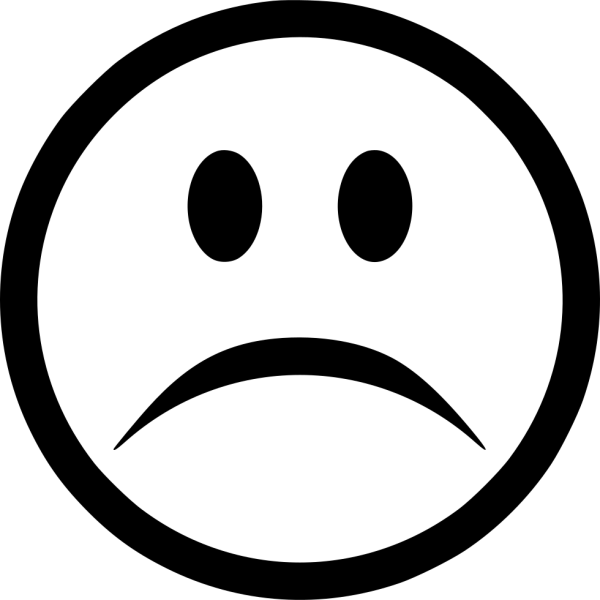
\includegraphics[width=0.483cm, height=0.36cm]{smile.png}   \\
 \hline
$-\infty$ & $-\infty$ & 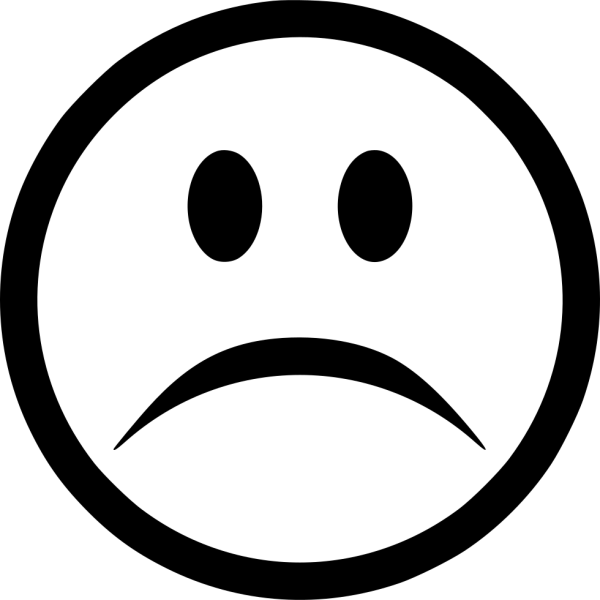
\includegraphics[width=0.483cm, height=0.36cm]{smile.png} & $\infty$    \\
 \hline
\end{tabular}
\qquad
\begin{tabular}{ |c|c|c|c| } 
 \hline
  $*$ & $a \in \mathbb{R} >0$ & $\infty$ & $-\infty$ \\
 \hline
 $b \in \mathbb{R} <0$ & $ab$ & $-\infty$ & $\infty$  \\
 \hline
 $\infty$ & $\infty$ & $\infty$ & $-\infty$   \\
 \hline
$-\infty$ & $-\infty$ & $-\infty$ & $\infty$    \\
 \hline
\end{tabular}
\end{center}
$0*\infty = $ $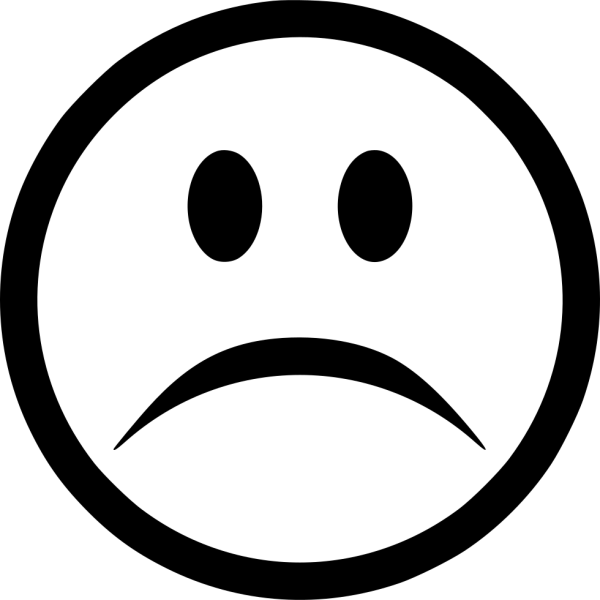
\includegraphics[width=0.533cm, height=0.4cm]{smile.png}$

когда-нибудь потом пригодится. Обозначим $\overline{\mathbb{R}}$

\deff{III. Аксиома Архимеда.}

$\forall x,y>0: \exists n \in \mathbb{N}:nx>y$

Следствие: Существует сколь угодно большие $\mathbb{N}$

Фан факт: мы не ввели $\mathbb{N}$. Но мы с ними работаем :)

\deff{IV. Аксиома Кантора.}

Пусть дана последовательность вложенных отрезков:

$[a_1,b_1] \supset [a_2,b_2] \supset \ldots$

Тогда пересечение этих отрезков не пусто.

Тогда наше $\mathbb{R}$ задается аксиомами I,II,III,IV.

\pagebreak

\section{Пределы и непр-сть отображений.}
\subsection{Предел. }
$(X,\rho^x),(Y,\rho^y): D \subset X$. $f:D \shortrightarrow Y$.

$a \in X, a$ - предельная точка D, $A \in Y$:

\deff{Предел отображения} $\lim\limits_{x\shortrightarrow a} f(x) = A$ - если выполнено любое из трех опр.

\begin{enumerate}
    \item $\epsilon-\delta$, по Коши: $\forall \epsilon>0 \exists \delta>0:\forall x\in D: \rho^x(x,a)<\delta : \rho^y(f(x),A)<\epsilon$.

    \item на языке окрестностей: $\forall U(A):\exists V(a): \forall x \in D \cap V(a)$ (V(a) в данном контексте проколотая, Кохась решил не говорить об этом): $f(x) \in U(A)$.

    \item по Гейне: $\forall(x_n): x_n \in D, x_n\shortrightarrow a, x_n \neq a: f(x_n) \shortrightarrow A$
    
\end{enumerate}

Частный случай. $X=Y=\mathbb{R}$, $D\subset \mathbb{R}, a \in \mathbb{R}, A 
\in \mathbb{R}$:

$\forall \epsilon >0: \exists \delta >0:\forall x \in D: 0<|x-a|<\delta: |f(x)-A|<\epsilon$

Зам:
\begin{enumerate}
    \item Опр. Гейне такие ($x_n$) существуют по свойствам предельной точки.
    \item Значение f(a) (если $a\in D$) никак не связана с величиной предела.
    \item Если $\exists U(a)$ f=g на $U(a)$, то они одновременно имеют общий предел/не имеют предел вовсе.
\end{enumerate}

\thmm{Теорема. Эквивалентность Коши и Гейне.} 

Опр. Коши $\Leftrightarrow$ Опр. Гейне.


\begin{enumerate}
        \item[] \uline{Доказательство.}
        
        Докажем $\Rightarrow$.  Берем $ x_n \in D, x_n\shortrightarrow a, x_n \neq a$. Проверим по опр. предела последовательности $f(x_n)\shortrightarrow A$.
        
        $\forall \epsilon>0 \exists \delta >0$.  Для этого $\delta : \exists N:\forall n > N: \rho(x_n,a)<\delta$.  $x_n \in D$, $x_n \neq a$. Для этих $x_n$ выполнено Коши $\rho (f(x_n),A)<\epsilon$. Откуда выполнено Гейне (пояснение: мы взяли последовательность из опр. Гейне и благодаря определению по Коши нашли предел)

        Докажем $\Leftarrow$. Дано $f(x_n) \shortrightarrow A$ по Гейне. Предположим, что A - не предел по Коши. 
        
        $\exists \epsilon >0: \forall \delta > 0: \exists x \in D, 0<p(x,a)<\delta: p(f(x),A) \geq \epsilon$. 
        Беру  $\delta=1, \exists x_1: \rho(x_1, a)<1$. Беру $\delta=\frac{1}{2}, \exists x_2: \rho(x_2, a)<1$.  Беру $\delta=\frac{1}{n},\exists x_n: \rho(x_n,a)<1$. Заметим, что последовательность $x_n$ удовлетворяет всем критериям Гейны($x_n \in D, x_n \neq a, x_n \shortrightarrow a$). Для нее $f(x_n) \shortrightarrow A$, тогда $\rho(f(x_n),A) \shortrightarrow 0$. Но у нас $\forall n: \rho(f(x_n),A)\geq\epsilon$. Противоречие.
\end{enumerate}

\thmm{Модификация определений.} (X,Y = $\mathbb{R}$  или $\overline{\mathbb{R}}$. )

1) $a \in \mathbb{R}$, $A = +\infty$, $X =\mathbb{R}$, $Y=\overline{\mathbb{R}}$. f: $D \shortrightarrow \overline{\mathbb{R}}$, $\lim\limits_{x\shortrightarrow a} f(x) = +\inf$. 

$\forall \epsilon \exists\delta>0: \forall x \in D, 0<|x-a|<\delta: f(x)>\epsilon$.

2) $ a = +\inf, A= - \inf$. $f: D\subset \mathbb{R} \shortrightarrow \overline{\mathbb{R}}$, $+\inf$,  - предельная точка D, $\lim\limits_{x\shortrightarrow a} f(x) = -\inf$. 

$\forall L \in \mathbb{R}: \exists \Delta: \forall x \in D: x>\Delta: f(x)<L$.

\deff{Метризуемая топология.}

Дана топология T в пр-ве X. (топология - совокупность открытых множеств). T метризуемая, если  $\exists$ метрика $\rho$, которая порождает эту систему открытых множеств.

\thmm{Теорема (о ед. пределе)}.

f: $D \subset X \shortrightarrow Y$, a - предельная точка D. $A,B \subset Y$.

$ {x_n\shortrightarrow a}: f(x) = A$ , ${x\shortrightarrow a}: f(x) = B$, тогда $A=B$. 

\begin{enumerate}
        \item[] \uline{Доказательство.}

        \sout{Очевидно по Гейне.}
                
         Распишем определение через окрестности и сделаем то же самое, что делали в других док-вах единтсвенности предела.
\end{enumerate}

\thmm{Теорема (о лок. ограниченности отображения, имеющего предел)}.

$f: D \subset X \shortrightarrow Y$, a - пр. точка D, $A \in Y$, ${x_n\shortrightarrow a},f(x_n) = A$. Тогда $\exists V(a): f|_{V(a)}$ - ограничена.

\begin{enumerate}
        \item[] \uline{Доказательство.}

        $U(a) = B(A,2025)$. Тогда $\exists V(a): \forall x \in D \cap V(a): f(x) \in B(A,2025)$. Если $a\in D$, возьму r = $max(\rho(A,f(a))+2025,2025)$ и буду делать шар радиуса не 2025, а радиуса R.
\end{enumerate}

\thmm{Теорема (о стабилизации знака)}.

$f: D \subset X \shortrightarrow Y$, a - пр. точка D, $\lim\limits_{x\shortrightarrow a} f(x) = A \in Y$, Пусть $B \in Y, B \neq A$. Тогда $\exists V(a): \forall x \in D \cap V(a): f(x) \neq B$.


\begin{enumerate}
        \item[] \uline{Доказательство.}

        $r= \cfrac{1}{2} \rho(A,B)$, для $U(A) = B(A,r) \exists V(a): \forall x \in D \cap V(a): f(x) \in B(A,r)$,  а следовательно $f(x) \neq B$.
\end{enumerate}

\thmm{Теорема} ( об арифм. свойствах предела).

X - м.п., Y - норм. $D \subset X$,$ f,g: D \shortrightarrow Y$, a - пр. точка D.

$A,B \in Y$, $f(x) \shortrightarrow A$, $g(x) \shortrightarrow B$, $ \lambda: D \shortrightarrow R: \lambda(x) \shortrightarrow \lambda_0 \in \mathbb{R}$, при $x \shortrightarrow a$.

Тогда  
\begin{enumerate}
    \item $f + g \shortrightarrow A + B$, при $x\shortrightarrow a$.
    \item $\lambda f \shortrightarrow \lambda_0 A$, при $x\shortrightarrow a$.
    \item $||f||\shortrightarrow ||A||$, при $x\shortrightarrow A$.
\end{enumerate}
\begin{enumerate}
        \item[] \uline{Доказательство.}
            ПО ГЕЙНЕ ОЧЕВ!!!
\end{enumerate}
\thmm{Теорема( об арифм. свойствах предела в $\mathbb{R}$)}.

$f: D\subset X \shortrightarrow \mathbb{R}$, a - пр. точка D, $f,g: D\shortrightarrow R$. $A,B \in \mathbb{R}$, $f(x) \shortrightarrow A$, $g(x) \shortrightarrow B$, при $x\shortrightarrow a$.

Тогда  
\begin{enumerate}
    \item $f + g \shortrightarrow A + B$, при $x\shortrightarrow a$.
    \item $f g \shortrightarrow AB$, при $x\shortrightarrow a$.
    \item $|f|\shortrightarrow |A|$, при $x\shortrightarrow A$.
    \item Если $B \neq 0$, то $\frac{f}{g}$=$\frac{A}{B}$. (Замечание: из-за теоремы о стабилизации знака, это корректно)
\end{enumerate}
\begin{enumerate}
        \item[] \uline{Доказательство.}
            Угадайте! По ГЕЙНЕ ОЧЕВИДНО.
\end{enumerate}















\thmm{Теорема (Предельный переход в неравенствах)}.

$f,g: D \subset X \shortrightarrow \mathbb{R}. a$ -  предельная точка D.

$f(x)\leq g(x) $ в $U(a) \cap D$ (выколотая окрестность). 

$\exists \lim\limits_{x\shortrightarrow a} f(x)=A \in \overline{\mathbb{R}}$,  $\exists \lim\limits_{x\shortrightarrow a} g(x)=B \in \overline{\mathbb{R}}$. Тогда $A \leq B$. Док-во по Гейне очевидно(так сказал Кохась, но мне вообще не очевидно).

\textbf{Зам.} $f(x)\leq g(x) \leq h(x)$.

Если $\exists \lim\limits_{x\shortrightarrow a} f(x)=A \in \overline{\mathbb{R}}$ и  $\exists \lim\limits_{x\shortrightarrow a} h(x)=A \in \overline{\mathbb{R}}$. 

То $g(x)$ имеет предел и он равен A.

\deff{Предел по мн-ве.} $f:D\subset X \shortrightarrow Y$. $D_1 \subset D$, $a$ - предельная точка $D_1$. Предел f при $x\shortrightarrow a$ по мн-ву $D_1$: $\lim \limits_{x\shortrightarrow a} f|D_1$

\deff{Односторонние пределы в $\mathbb{R}$.}

$\lim\limits_{a+0} f(x)$ - предел правосторонний 

$\lim\limits_{a-0} f(x)$ - предел левосторонний 

\thmm{Теорема о пределе монот. f}:

f: $D \subset \mathbb{R} \shortrightarrow \mathbb{R}$ монотонная. Пусть есть $a \in \overline{\mathbb{R}}$. $D_1 = (-\infty, a) \cap D$, a  -предельная точка.
\begin{enumerate}
    \item f - возрастает, огр сверху. Тогда $\exists \lim\limits_{x \shortrightarrow a - 0} f(x)$
    \item f - убывает, огр. снизучё. Тогда $\lim_{x\shortrightarrow a-0} f(x)$ - существует и конечен.
\end{enumerate}
Доказательство аналогично т.о пределе монотонной послежовательности.
\pagebreak
\subsection{Компактность.}

\thmm{Лемма Гейне-Борели.}

$ [a,b] \subset \bigcup\limits_{i=1}^{\infty} (a_i,b_i)$. Тогда $\exists$ кон. число интервалов, что $ [a,b] \subset \bigcup\limits_{i=1}^{n} (a_i,b_i)$.

Я не буду доказывать эту лемму, она сама потом докажется

\textbf{Опр.} X - метр. пр-во, $K \subset X$, K - \deff{компактно} в X, если из любого отрытого покрытия множества K, можно выбрать конечное подпокрытие.

$\forall (G_{\alpha})_{\alpha \in A}$ - откр в X, $K \subset \bigcup\limits_{\alpha \in A} (G_\alpha)$. $\exists$ конечное $\alpha_1,\ldots,\alpha_n$, что $K \subset \bigcup\limits_{i=1}^n (G_{\alpha_i})$.

\thmm{Теорема.}

$K \subset Y \subset X$ (($Y,\rho$) - подпространство ($X,\rho$)).

Тогда, если K компактно в Y, то это \textbf{равносильно} K - компактно в X.

\begin{enumerate}
        \item[] \uline{Доказательство.}

        \uline{Докажем в правую сторону}. Если K - компактно в Y, то должно быть. что K - в X.  Берем произвольное открытое покрытие. (Обознаю $G_\alpha^X$ - открытое в X,  $G_\alpha^Y$ - открытое в Y)
        
        $K \subset \bigcup\limits_{\alpha \in A} (G_\alpha^X)$. Хотим доказать, что можно выбрать конечное подпокрытие.

         $K \subset \bigcup\limits_{\alpha \in A} (G_\alpha^X) \cap Y =  K \subset \bigcup\limits_{\alpha \in A} (G_\alpha^X \cap Y).$ По закону Де-Моргана.

        $K \subset \bigcup\limits_{\alpha \in A} (G_\alpha^X \cap Y). = K \subset \bigcup\limits_{\alpha \in A} (G_\alpha^Y)$, для этого покрытия существует конечное, тк K компактно в Y. 

         $K \subset \bigcup\limits_{i=1}^n (G_{\alpha_i}^Y)\subset \bigcup\limits_{i=1}^n (G_{\alpha_i}^X)$. Откуда получаю, что из любого покрытия, можно выбрать конечно подпокрытие, откуда K компактно в X. 

         \uline{Докажем в левую сторону}. Дано K компатно в X. Возьму произвольное открытое  покрытие. $K \subset \bigcup\limits_{\alpha \in A} (G_\alpha^Y)$, хочу доказать, что можно выбрать конечное подпокрытие.

         Каждому $G_\alpha^Y$   можно задать $G_\alpha^X$, такой, что $G_\alpha^Y = G_\alpha^X \cap Y$.

         Возьму получившееся семейство. Очевидно, что $ K \subset \bigcup\limits_{\alpha \in A} (G_\alpha^X)$, по определению компактности в X есть конечное подпокрытие $K \subset\bigcup\limits_{i=1}^n (G_{\alpha_i}^X)$.

         Пересеку его с Y. Получу $K \subset \bigcup\limits_{i=1}^n (G_{\alpha_i}^X \cap Y )= \bigcup\limits_{i=1}^n (G_{\alpha_i}^Y)$, откуда получаю, что из любого покрытия, я могу выбрать конечное, откуда K компактно в Y. Q.E.D. 
\end{enumerate}

\textbf{Замечание от Славы:} Тк мы доказали предыдущую теорему, то мы можем употреблять компактность без уточнения множества. В дальнейшем, вместо K компактно в X будет употребляться K компактно.

\thmm{Теорема}.

Пусть $(X,\rho)$, $K\subset X$.

\begin{enumerate}
    \item K - компактно $\Rightarrow$ K - замкнуто и ограниченно.
    \item X - компактно, K - замкнуто $\Rightarrow$ K - компактно.
\end{enumerate}

\begin{enumerate}
        \item[] \uline{Доказательство.}
        
       \textbf{ 1a) Дано K - компактно. Докажем, что K - замкнуто.} 
        
        Чтобы доказать, что что-то замкнуто, мы доказываем, что дополнение открыто.

        Доказать $K^c$ - открыто, т.е. $\forall a \in K^c$ a должно быть внутренней.

        $K \subset \bigcup\limits_{x \in K} B(x,\frac{1}{10}\rho(a,x))$. По определению компактности  существуют $x_1,\ldots,x_n$, такие  
        
        $K \subset \bigcup\limits_{i=1}^{n} B(x_i,\frac{1}{10}\rho(a,x_i))$.

        И суть в том, что $ B(x_i,\frac{1}{10}\rho(a,x_i)$ и $B(a,\frac{1}{10}\rho(a,x_i)$ не пересекаются!

        Возьму $ r = min(\frac{1}{10}\rho(x_i,a))$. так как x-ов конечно, то такой минимум есть. Тогда B(a,r) не пересекается с K, откуда он лежит в $K^c$, откуда дополнение открыто.

        \textbf{Замечание от Славы.} Для каждой точки дополнения у нас существует окрестность в которой она лежит, откуда по определению каждая точка дополнения K - внутренняя, откуда дополнение K открыто.
        
        \textbf{1б) Дано K - компактно. Докажем, что K - ограниченно.} 

        Возьму $a\in X$. Тогда $K\subset \bigcup\limits_{n=1}^{\infty} В(a,n) = X$. Так как K компактно, то существуют  такие $x_1,\ldots,x_n$, $K\subset \bigcup\limits_{i=1}^{l} В(a,n_i)=B(a,n_l)$, откуда получаю искомое.

        \textbf{Замечание от Славы.} Множество K лежит в шаре $B(a,n_l)$, откуда  оно ограниченно этим шаром.
        
        \textbf{2) Проверим, что K - компактно.} 

        Возьмем какое-то покрытие:$K \subset \bigcup\limits_{\alpha \in A} (G_\alpha)$, хочу доказать, что можно выбрать конечное подпокрытие.
        
        $\bigcup\limits_{\alpha \in A} (G_\alpha) \cup K^c$. Заметим, что т.к. K - замкнуто, то $K^c$ открыто и является покрытием X.
        
        Так как X компактно, то существуют  такие $x_1,\ldots,x_n$, что $X \subset  \bigcup\limits_{i=1}^{n} G_{\alpha} \cup K^c$.

        $K \subset X \subset  \bigcup\limits_{i=1}^{n} G_{\alpha} \cup K^c$, но тк $K$ и $K^c$ не пересекаются, то
        
       $K \subset \bigcup\limits_{i=1}^{n} G_{\alpha}$.  Откуда получаю, что из любого покрытия, я могу выбрать конечное, откуда K компактно Q.E.D. 
\end{enumerate}
\deff{Параллелепипед.}

$\{x \in \mathbb{R}^m: \forall k = 1\ldots m: a_k\leq x_k \leq b_k\}$ --- такое множество называется параллелепипедом, обозначается
$[a,b]$, где$ a,b \in \mathbb{R}^m$. 

\deff{Лемма(о вложенных параллелепипедах)}.

Здесь индексы обозначаются сверху.


$[a^1,b^1]\supset [a^2,b^2]\supset \ldots$ --- последовательность парал. в $\mathbb{R}^m$.

Тогда $\bigcap\limits_{k=1}^{\infty} [a^k,b^k]$ --- не пусто.

\begin{enumerate}
        \item[] \uline{Доказательство.}
        
       \sout{как сказал кохась - очевидно.}

       Используем аксиому Кантора для каждой координаты и получим итоговое.
\end{enumerate}

\thmm{Лемма}.

Дан замкнутый прлп. [a,b] в $\mathbb{R}^m$. Докажем, что он компактный.
\begin{enumerate}
        \item[] \uline{Доказательство.}


        $[a^1,b^1] \subset \bigcup\limits_{\alpha \in A} (G_\alpha) $. $diam[a^1,b^1]=||b^1-a^1||$
        
        Предположим, что не сущ. конечного подпокрытия. Разобьем мой прпл. на $2^n$ - половинных прпл. Следовательно найдется половинный прпл. $[a^2,b^2]$, для которого нельзя выбрать конечное подпокрытие.

        Давайте теперь продолжу выполнять этот процесс. Найдутся $[a^4,b^4],[a^5,b^5],\ldots$.

        $[a^1,b^1]\supset [a^2,b^2]\supset \ldots$ --- последовательность прпл. в $\mathbb{R}^m$. $diam[a^k,b^k]=\frac{||b^1-a^1||}{2^k}$.

        По предыдущей лемме $\exists x \in \bigcap\limits_{k=1}^{\infty} [a^k,b^k] \subset [a^1,b^1]$. 

           $x\subset \bigcup\limits_{\alpha \in A} (G_\alpha)$, значит есть какой-то $\alpha_0$, что $x\in G_{\alpha_0}$. Тогда $\exists r>0 B(x,r)$. И тк диаметр $a^k,b^k$ стремится к нулю, то в какой-то момент этот шарик покроет прпл. $a^l,b^l$. Тогда приходим к противоречию. Q.E.D

           \textbf{Замечание от Славы.} Мы предполагаем, что нельзя, тогда не должно существовать таких шариков, покрывающих один из бесконечнего кол-ва прпл (которые нельзя покрыть конечным числом шариков), а такой есть.
\end{enumerate}

\thmm{Теорема ( о характеристике компактности в $R^m$)}

Эквиваленты утверждения:
\begin{enumerate}
    \item $K \in R^m$ - замкнуто и ограничено. 
    \item $K$ - компактно.
    \item $K \in R^m$ - \textbf{секвенциально компактно}, т.е. $\forall (x_n)$ - посл. в K, $\exists (n_k):n_1<n_2<\ldots$ - посл нат чисел, $\exists a\in K$: $x_{n_k} \shortrightarrow a$.
\end{enumerate}
\begin{enumerate}
        \item[] \uline{Доказательство.}
        
        \uline{Из первого второе}. 
        
        Пусть $K \in R^m$ - замкнуто и ограничено. Тогда $\exists$ прпл. [a,b]: $K \subset [a,b]$. причем K - замкнуто. Значит по лемме (см. наверх), наш прпл. компактный, а по теореме(см наверх) значит, что и K - компактно.

        \uline{Из второго третье.} 

        $x_n$ - посл. в K. D = ${x_n} \subset K$, причем в D нет повторений.
        
        Если D конечно, то какое-то значение принимается бесконечное кол-во раз, выберем только их и получим то, что от нас требуется.

        Если D бесконечно. Если $\exists$ a - предельная точка $D$, лежащая в K, тогда такая последовательность строится очевидно. 
        
        Если таких нет. Тогда $K \subset \bigcup\limits_{x \in K} B(x,\varepsilon_x) $. Так как никакая из точек в K - не предельная для D, то каждую точку, я могу окружить шаром, что в нем не будет ни одного элемента D. ($\varepsilon_x$ я выбираю именно так). 
        
         $D \subset K \subset \bigcup\limits_{1}^{n} B(x,\varepsilon_x) $ не более n точек из D. Тогда не существует конечного покрытия. 
 Противоречие. 

        \uline{Из третьего первое.} Проверим, что K - замкнуто. Если нет, тогда $\exists a \notin K$, a - предельная точка K. Тогда $\exists (x_n)$ - посл. в K. $x_n \shortrightarrow a$. $\forall (n_k) x_{n_k}$ сходится к $a\in K$, по секвенциальной компактности.
\end{enumerate}

\thmm{Следствие (Принцип выбора Больцано-Вейерштрасса)}.

в $\mathbb{R}^m$ $x_n$ - огр. последовательность. $\exists (n_k)$, такое, что $x_{n_k}$ сходится.

\begin{enumerate}
        \item[] \uline{Доказательство.}
        
       $(x_n)$ - огр., значит он лежит в каком-то парал [a,b], который компактен, а если он компактен, то по характеристике компактности он секвенциально компактен, откуда и следует искомое. Q.E.D.
\end{enumerate}

Опр. $(X, \rho)$  - м. п, ($x_n$) - посл-ть в X
$(x_n)$ - \deff{фундаментальная} = после-ть Коши = сходящаяся в себе, если
$\forall \varepsilon > 0: \exists N: \forall m,n>N: \rho(x_m,x_n)<\varepsilon$.

\thmm{Лемма.} $(X, \rho)$  - м. п
\begin{enumerate}
    \item $(x_n)$ - посл. Коши, то $(x_n)$ - огр.
    \item $(x_n)$ - посл. Коши, $\exists(n_k): x_{n_k}$ - возрастающая и сходится, то $(x_n)$ - сходится
\end{enumerate}

\begin{enumerate}
        \item[] \uline{Доказательство.}
        
        1) Возьмем $\varepsilon = 1$, $ \exists N: \forall m,n>N: \rho(x_m,x_n)<1$. Возьму $n_0>N$. Заметим, что $\forall n>N: n \in B(x_{n_0},1)$. Возьму r=max($\rho(x_{n_0},x_i)$), где i от 0 до N и сделаю шар радиуса R=max(r+1,1). Тогда все точки попадут в него откуда $(x_n)$ - огр.

        2) $\forall \varepsilon>0: \exists N: \forall m,n>N \rho(x_m,x_n)<\frac{\varepsilon}{2}$ 
        и также $\exists K:\forall b>K:\rho(x_{n_b},a)<\frac{\varepsilon}{2}$.  Возьмем M = max(N,K). $\forall m > M\rho(x_m,a)<\rho(x_m,x_{n_m})+\rho(x_{n_m},a)<\varepsilon$. Откуда сходится. Q.E.D
\end{enumerate}

\deff{Фундоментальная последовательность.} $(X,\rho)$ - метрическое пространство, $x_n$ - последовательность в X. Последовательность фундаментальна, если $\forall \varepsilon >0 \exists N, \forall m,n > N: \rho(x_n,x_m)<\varepsilon$. Такая последовательность  называется последовательностью Коши.

\textbf{Лемма.}  ${x_n}$ -  посследовательность в $(X,\rho)$.

\begin{enumerate}
    \item $x_n$ посл. Коши и $x_n$ ограниченно.
    \item $x_n$ посл Коши и есть $x_{n_k}$, которое сходится,  то $x_n$ сходится.
\end{enumerate}
Доказательство очевидно.

\deff{Полное пространство} - любая фунд. последовательность в нем сходится. 

Антипример: $x_n = \frac{1}{n}$ в $(0,+\infty)$. Пример: $R^m$.

В полном пространстве: фундоментальная = сходится и наоборот.

\deff{Критерий Больцмана-Коши.} (существования предела в полном пространстве)

$\exists \lim\limits_{n\shortrightarrow +\infty} x_n = a \Leftrightarrow \forall \varepsilon>0 \, \exists N: \forall n,m > N:\rho(x_n,x_m)<\varepsilon$

\thmm{Теорема. Критерий Больцмана-Коши для отображений.}

Пусть есть $D \subset X \shortrightarrow Y$, X,Y - метрические пространства. $x_0$ - предельная точка D. Y - полное, тогда имеет место:
\begin{enumerate}
    \item $\exists \lim_{x\shortrightarrow x_0} f(x) $
    \item $\forall \varepsilon>0: \exists \delta >0: \forall x_1,x_2 \in D\textbackslash\{x_0\}: 
    \begin{cases}
         \rho(x_1,x_0)<\delta \\
         \rho(x_2,x_0)<\delta
    \end{cases}
     \rho(f(x_1),f(x_2))<\varepsilon$
\end{enumerate}

\begin{enumerate}
    \item[] \prooff{}
    Доказательство в правую сторону очевидно. Доказываем в левую сторону.
    Воспользуемся \deff{пределом по Гейне}. Возьму $x_n \shortrightarrow x_0$, $x_n \in D$, $x_n \neq x_0$. f($x_n$) - фундоментально из правой части (расписать и посмотреть). А так как фундоментально,то значит сходится по Критерию Больцмана-Коши.
\end{enumerate}

\pagebreak
\subsection{Непрерывные отображения.} 

$f: D \in X \shortrightarrow Y, x_0 \in D$, Y,X - метрические пространства.
f \deff{непрерывна} в $x_0$, если выполнено 1 из 4:
\begin{enumerate}
    \item $\exists \lim\limits_{x\shortrightarrow x_0} f(x) = f(x_0)$, либо $x_0$ - изолированная.
    \item По Коши.$\forall \varepsilon>0:\exists \delta>0: \forall x\in D: \rho (x,x_0)<\delta$,$\rho(f(x),f(x_0))<\varepsilon$
    \item Окр. $\forall U(f(x_0)):\exists V(x_0): \forall x \in D \cap V(x_0): f(x_0) \in U(f(x_0))$
    \item По Гейне. $\forall (x_n): x_n \shortrightarrow x_0, x_n \in D: f(x_n) \shortrightarrow f(x_0)$
\end{enumerate}

Случай в $R$:   $\forall \varepsilon>0:\exists \delta>0: \forall x \in D: |x-x_0|<\delta: |f(x)-f(x_0)|<\varepsilon$.

\deff{Разрывная} в $x_0$ - нет непрерывности. (f терпит разрыв в $x_0$). В таком случае $x_0$ - \deff{точка разрыва}. 

Также в $\mathbb{R}$ можно ввести непрерывность \textbf{слева} и \textbf{справа}. (меняем пределы на левосторонний и правый).

Если функция непрерывна справа и слева от $x_0$, то она непрерывна.

Введем обозначение. $f(x\pm0)=\lim\limits_{x\shortrightarrow x_0 \pm 0}f(x)$.

Если $f(x_0-0),f(x_0),f(x_0+0)$ не все совпадают(если существуют и конечны), тогда $x_0$ - \deff{точка скачка} или разрыва первого рода.

Все другие - разрывы второго рода (не могу вычислить левосторонний предел или правостронний).


\deff{Свойства непрерывного отображения.}

\textbf{Арифметические свойства:}

\thmm{Теорема.}

f, g: $D \subset X \shortrightarrow Y$, X - метрическое пространство, Y - нормированное, $x_0 \in D$. $\lambda: D \shortrightarrow \mathbb{R}$, f, g, $\lambda$ - непрерывны в $x_0$. 

Тогда f+g, $\lambda f$, $||f||$ - непрерывны в $x_0$. Доказательство очевидно из арифм. свойств предела.

\thmm{Теорема.}

f, g: $D \subset X \shortrightarrow \mathbb{R}$, X - метрическое пространство, $x_0 \in D$, f,g - непрерывны в $x_0$. 

Тогда f+g, fg, |f| - непрерывны в $x_0$, а также, если $g(x_0)\neq 0: \cfrac{f}{g}$ - непрерывна в $x_0$. Доказательство очевидно из арифм. свойств предела в $\mathbb{R}$.

\textbf{Стабилизация знака.}

$f: D \subset X \shortrightarrow \mathbb{R}, x_0 \in D, f(x_0)\neq 0.$, $f(x)$ непрерывна в $x_0$.

Тогда $\exists U(x_0): \forall x \in U(x_0): $ sign $ f(x) = $ sign $f(x_0)$.

(Пересказ теоремы о стабилизации знака).

Функция называется \deff{непрерывной}, если она непрерывны в любой своей точке, то есть $f: D \subset X \shortrightarrow Y$, и f непрерывна в D, если $\forall x_0 \in D: f$ непрерывна в $x_0$.




\thmm{Теорема.(непрерывность композиции)}

$f: D \subset X \shortrightarrow Y, g: E \in Y \shortrightarrow Z$, $f(D) \subset X.$ f - непрерывна  в $x_0 \in D$, g - непрерывна а $f(x_0)$. Тогда $g(f(x)) $ непрерывна в $x_0$.

\begin{enumerate}
    \item[] \prooff{}
    \sout{Доказательство состоит из волшебных слов: по Гейне.}

    Надо проверить, что $\lim\limits_{x \shortrightarrow x_0} g(f(x)) \shortrightarrow g(f(x))$. Возьмем $x_n \shortrightarrow x_0, x_n \in D. f(x_n) \shortrightarrow f(x_0)$, тк.f непрерывна. Есть некая $f(x_n) \shortrightarrow x_0$. Теперь воспользуемся непрерывности g и получим искомое.
\end{enumerate}

\thmm{Теорема. (о пределе композиции)}

$f: D \subset X \shortrightarrow Y, g: E \in Y \shortrightarrow Z$, $f(D) \subset X. \lim\limits_{x\shortrightarrow a}f(x) = b, \lim\limits_{y\shortrightarrow b} g(y) = L$. Тогда:
$\lim\limits_{x\shortrightarrow a} g(f(x)) = L$

Если выполнено одно из двух:
\begin{enumerate}
    \item g - непрерывна в точке b.
    \item $\exists U(a): \forall x \in U(a) \cap D: f(x) \neq b$.
\end{enumerate}

\begin{enumerate}
    \item[] \prooff{}
    Кохась сказал, что это упражнение. Позже тут появится док-во, честно-честно (док-во вообще следует из прошлой задачи, если я умею думать)
\end{enumerate}

% Кохась сказал, что здесь еще будет что-то

\thmm{Теорема. ( о топ. определении непрерывности)}

$f: X \shortrightarrow Y$, X,Y - метрическое пространство. Тогда эквивалентно:
\begin{enumerate}
    \item f - непрерывно на X
    \item $\forall G \subset Y$, G - откр в Y: $f^{-1}(G)$ - открыто в X.
\end{enumerate}

\begin{enumerate}
    \item[] \prooff{}
    Из первого второе. Возьму $G \subset Y$ - открытое. Проверим, что $f^{-1}(G)$ - открытое.

    $\forall x_0 \in f^{-1}(G)$ Проверим, что $x_0$ - внутренняя точка $f^{-1}(G)$. \sout{очевидно.} f непрерывно в $x_0$, значит, что $\forall K$ - открытой в Y, существует открытая H, $x_0 \in H$: $\forall x \in H \in D: f(x) \in K$. что и доказывает нужное нам.

    Из второго первое. Возьму $f(x_0) \in G$. Непрерывность в $x_0$ означает, что верно ли: $\forall G_1$ - открытой $f(x_0) \in G_1 \exists$ открытая H, $x_0 \in H: H \subset f^{-1}(G_1)$. Исходя из того что дано это выполнено
\end{enumerate}
%todo: подумать

\thmm{Теорема. (Вейерштрассса)}

$f: X \shortrightarrow Y$, где X,Y - метрические пространства - непрерывно.

$X$ компактно. Тогда f(X) - компактно.

\begin{enumerate}
    \item[] \prooff{}
    Проверим, что f(X) - компактно.

    Возьму любое покрытие $f(X) \subset \bigcup\limits_{\alpha \in A} G_\alpha$, где $G_\alpha$ - открытое в Y. Надо доказать, что я могу выбрать конечное подпокрытие.

    $X \subset \bigcup\limits_{\alpha \in A} f(G_{\alpha})$. по теореме о топ. определении каждый прообраз открыт. Откуда, тк X компактно,  можно выбрать конечное
    $X \subset \bigcup\limits_{i=1}^n f^{-1}(G_{\alpha_i})$.
    Тогда $f(X) \subset \bigcup\limits_{i=1}^n G_{\alpha_i}$, откуда получаем искомое
    
\end{enumerate}

\textbf{Следствие}

$f: X \shortrightarrow Y, f$ - непрерывно на X, X - компактно, тогда f(x) замкнут и ограничен в Y.

\textbf{Следствие (1-ая теорема Вейерштрасса)}

$f: [a,b] \shortrightarrow \mathbb{R}$, непрерывна. Тогда f - огр на [a,b].

\textbf{Следствие}

$f: X \shortrightarrow \mathbb{R}$. X - компактен, f - непрерывна. Тогда есть максимум и минимум функции.

\begin{enumerate}
    \item[] \prooff{}
    f(X) замкнуто и ограниченно в $\mathbb{R}$.$\sup(f(x),x\in X)$. Если супремум не бесконечность, но $\sup f(x) \notin f(x)$, тогда $\sup f(x)$ - предельная из технического описания супремума . А откуда наше множество не замкнуто - Противоречие. Для минимума аналогично.
\end{enumerate}

\textbf{Следствие (Главная теорема Вейерштрасса)}
%TODO: точки

$f: [a,b]\shortrightarrow \mathbb{R}$, непрерывная, тогда существует max и min. 

ИСПОЛЬЗУЕМ МАТЕМАТИЧЕСКУЮ ТЕРМИНОЛОГИЮ --- \textbf{ЯСЕН ПЕНЬ ОЧЕВИДНО}.




$\mathbb{R}$ - $\varphi: [a,b] \shortrightarrow \mathbb{R}^m$, непрерывное - такое называют путем при течении времени от a до b.

Множество $E \subset \mathbb{R}^n$,  называют \deff{линейно связным}, если любые две точки можно соединить путем.

$\forall A, B \in E$. $\exists \varphi: [a,b] \shortrightarrow E $, непрерывно, что $\varphi(a)= A, \varphi(b) = B$.

\deff{Связное множество} Е в $R^m$ ---  если его нельзя представить в виде двух непересекающихся открытых в E множеств и не пустые в пересечении с $E$.

Утв. \thmm{Теорема.}

$[a,b] \subset \mathbb{R}$. Тогда $[a,b]$ - связно. 

Не существует: $G_1,G_2$ - открытые в $\mathbb{R}$, что пересечение не пусто. $G_1 \cap G_2 \neq 0$ и $[a,b] \subset G_1 \cup  G_2  $

\begin{enumerate}
    \item[] \prooff{}
    Докажем от противного. Пусть существует такие $G_1,G_2$. Тогда Н.У.О $a \in G_1$ и $b \in G_2$. $s:= \sup(x: [a,x] \subset G_1) \leq b$. $s > a$.
    Куда принадлежит $s$? Пусть принадлежит $G_1$, но тогда $s_1$ - внутренняя, откуда справа от точки что-то есть, а там ничего нет, потому что она супремум. Пусть $s$ лежит в $G_2$. Тогда супремум чуть левее. Противоречие.
\end{enumerate}

\textbf{Замечание от Славы.} Лучше для понимания верхней штуки порисовкать рисуночки и подумать.

\thmm{Теорема (Больцмана-Коши о промежуточном значении)}.

$f: [a,b] \shortrightarrow \mathbb{R}$. f - непрерывная. Тогда $\forall t$ между $f(a),f(b)$, для которой $f(c) = t$, где $c \in [a,b]$.

\begin{enumerate}
    \item[] \prooff{}
    Допустим, что не так. Тогда есть какое-то t, которое не представимо(если больше, то более очевидно). Тогда отрезок $[a,b] = f^{-1}((\infty,t)) \cup f^{-1}((t,+\infty))$. Получается, что я отрезок a,b представил в виде двух открытых множеств. По прошлой теореме я проиграл.
\end{enumerate}

\textbf{Пример}. Теорема о Бутерброде. Для двух любых открытых множеств в $\mathbb{R}^2$. можно провести прямую, которая поделить каждое множество на 2 равных по площади части.

\textbf{Тут Слава забыл расписать доказательство, я его подменю.} Заведите параметр $a$ - угол наклона прямой. Для любого угла наклона можно найти такую прямую, что поделит первое множество пополам(по прошлой теореме). Можно завести отображение $f : a \rightarrow \mathbb{R}$ равное площади второго множеста слева от прямой, из которой вычли площадь второго множества справа от прямой(для этого задайти лево и право для прямой). Заметим, что при повороте $a$ с 0 до 180 градусов это непрерывное значение поменяло знак. Снова пользуемся прошлой теоремой(тут нужно сказать, что $f$ непрерывно) и получаем, что существует такое $a$, при котором оба множества делятся пополам.

\textbf{Замечание от Кохася:} Введем новое обозначение $\sqcup$ - дизъюнктное объединение. Также введем $\textquotestraightdblbase[a,b]\textquotestraightdblbase$ - отрезок от a до b или от b до a (мы не знаем кто больше)

\thmm{Теорема (о сохранении промежутка)}

$f: \langle a,b \rangle \shortrightarrow \mathbb{R}, f $ - непр. Тогда $f(\langle a,b \rangle)$ - промежуток.
\begin{enumerate}
    \item[] \prooff{}
    Давайте возьмем  $m = \inf f, M = \sup f$ на промежутке $\langle a,b \rangle$. Достаточно проверить, что $(m,M) \subset f( \langle a,b \rangle )$.  Возьмем t на промежутке. $m<t$,  Тогда существует $x_1 \in \langle a,b \rangle : f(x_1)<t$. $M>t$  $x_2 \in  \langle a,b \rangle; f(x_2)>t$. Тогда по теореме Больцмана-Коши существует такое c, что $f(c) =t$. Q.E.D 
\end{enumerate}

\textbf{Напоминание:} $\langle a,b \rangle$ - нам все равно включительно или нет границы.

\textbf{Лемма.} $E \subset \mathbb{R}$ - линейно связно равносильно тому, что E - промежуток. 

\begin{enumerate}
    \item[] \prooff{}
    Из правого левое - по прошлой теореме.

    В обратную сторону.  Положим $m = \inf E, M = \sup E$. Закончите сами  %Todo: доделать
\end{enumerate}

\thmm{Теорема (Больцмана-Коши о сохранении линейной связности)}.

$X - $лин. связное м.п., $Y$ - метрическое пространство $f: X \shortrightarrow Y$ - непрерывно. Тогда $f(X)$ - линейно связное множество.
\begin{enumerate}
    \item[] \prooff{}
   Беру A, B. $f(a) = A, f(b) = B$ из f(X). $\exists \gamma: [\alpha,\beta] \shortrightarrow X$ - непр. Такое, что. $f \cdot g [a,b] \shortrightarrow Y$ - непрерывно.
\end{enumerate}

Кохась написал что-то странное надо переделать

%TODO

\thmm{Теорема (о непрерывности монотонной функции)}

$f: \langle a,b\rangle \shortrightarrow \mathbb{R}$ монотонна. 

\begin{enumerate}
    \item Тогда f не имеет разрыва второго рода.
     Т.е. $\forall x: \exists f(x-0), f(x+0)$ [ну почти]
     \item f - непр $\Leftrightarrow f(\langle a,b\rangle)$ - промежуток \textbf{Волшебное утв.}
\end{enumerate}

\begin{enumerate}
    \item[] \prooff{}
   1) Н.У.О f - возрастающая. Тогда фикс. $x\in (a,b)$. Пусть $x_1,x_2\in (a,b): x1<x<x2$. $f(x-0)=\lim\limits_{x_1\shortrightarrow x-0} f(x_1)$. По теореме о пределе монотонной функции и при этом предел не превосходит f(x). Аналогично правосторонний

   2) вправо уже доказывали(см выше). Докажем влево. Берем $x_0$ на промежутке. Левосторонний равен правостороннему предел, что очевидно из того, что это промежуток.   
\end{enumerate}

Следствие. $f:<a,b> \shortrightarrow \mathbb{R}$ - монотон.
Тогда число точек разрыва не более чем счетно. (Сделать инъекцию в множество $\mathbb{Q}$ и победили).

\thmm{Теорема (о сущ. непрерывности обратной функции)}.

$f: \langle a,b \rangle \shortrightarrow \mathbb{R}$ непрерывна и строго монотонна.

$m = \inf f, M = \sup f$. Тогда:

\begin{enumerate}
    \item $f$ обратима. $f^{-1} \langle m,M\rangle \rightarrow \langle a,b \rangle$. биекция*
    \item $f^{-1}$ того же вида монотонности, что и f
    \item $f^{-1}$ непрерывен.
\end{enumerate}

\begin{enumerate}
    \item[] \prooff{}
    Пусть $f$ - строго возрастает. $\langle m, M\rangle $, того же вида, что и $\langle a, b \rangle $. $f: \langle a,b \rangle \rightarrow \langle m ,M \rangle $~--- биекция. Второе очевидно. а непрерывна по теореме о непрерывности о монотонной функции. 
\end{enumerate}





   
\pagebreak
\section{Асимптотические оценки.}

\subsection{Оценки}
Введем \textbf{обозначения}:


$f,g: D \subset X \shortrightarrow \mathbb{R}, x_0$ - предельная точка D.

Если $\exists U(x_0)$; $\exists \varphi: D \shortrightarrow \mathbb{R}$ : $f(x) = \varphi(x)g(x)$:

Если:
\begin{enumerate}
    \item $\varphi$ - ограниченная на $U(x_0) \cap D$, то f = $O$(g) ($U(x_0)$ вроде выколотая окрестность)
    \item $\varphi(x) \shortrightarrow 0$, при $x\shortrightarrow x_0$, то $ f = o(g)$
    \item $\varphi \shortrightarrow 1$, то $f $\mytilde$ g$ --- эквивалентность при $x \shortrightarrow x_0$.
\end{enumerate}

$f,g: D \subset X \shortrightarrow \mathbb{R}: \exists c>0: \forall x \in D : |f(x)|\leq c g|(x)|$. Тогда $f = O(g)$.

$f = O(g); g = O(f).$ Тогда $f \asymp g$, называются \textbf{сравнимыми}.


\deff{Замечания:}

\begin{enumerate}
    \item $\cfrac{f}{g}$ - огр. на  $U(x_1) \cap D$. Тогда $f = O(g)$
    \item $\cfrac{f}{g}  \shortrightarrow 0 \Rightarrow f= o(g),$ при $x\shortrightarrow x_0$.
    \item $\cfrac{f}{g}  \shortrightarrow 1 \Rightarrow f$\mytilde$g,$ при $x\shortrightarrow x_0$.
\end{enumerate}

$O$(g), $o$(g)  будут использоваться как классы функций (множество).

\sout{про что дядя кохась не сказал.}

\deff{Свойства:}
\begin{enumerate}
    \item $o(f) + o(f) = o(f)$. $o(f) - o(f) = o(f)$.
    \item \textbf{Принцип Тортика.} $f$\mytilde$g \Leftrightarrow f = g + o(g)$$\Leftrightarrow f = g + o(f)$.
    \item $f = o(g) \Rightarrow f = O(g)$.
\end{enumerate}

\sout{Кохась ругает нас за работу}

\textbf{Таблица эквивалентности}, при $x\shortrightarrow 0$.

\begin{enumerate}
    \item $\sin x $ \mytilde $ x$
    \item $\tg x $ \mytilde $ x$
    \item $\arcsin x $ \mytilde $ x$
    \item $\arctg x $ \mytilde $ x$
    \item $\cos x $ \mytilde $ 1$
    \item $1 - \cos x $ \mytilde $ \cfrac{x^2}{2}$
    \item $e^x-1 $ \mytilde $ x$
    \item $a^x-1 $ \mytilde $ x \ln a$
    \item $\ln (1+x)$ \mytilde $x$
    \item $(1+x)^\alpha -1$ \mytilde $\alpha x$, $\alpha \in \mathbb{R}$
    
\end{enumerate}

\thmm{Теорема. (о замене на эквивалентное)}

$f,\tilde{f},g,\tilde{g}: D \subset X \shortrightarrow \mathbb{R}$, X - метрическое пространство. $x_0$ - предельная точка D.\,\, $f$ \mytilde $\tilde{f}$, $g$ \mytilde $\tilde{g}$.

Тогда $\lim\limits_{x\shortrightarrow x_0} f(x)g(x) = \lim\limits_{x\shortrightarrow x_0} \tilde{f}(x) \tilde{g(x)}$ и $\lim\limits_{x\shortrightarrow x_0} \cfrac{f(x)}{g(x)} = \lim\limits_{x\shortrightarrow x_0} \cfrac{\tilde{f}(x)}{ \tilde{g(x)}}$. 

Если $x_0$ - предельная точка $\cfrac{f(x)}{g(x)}$ и если существует предел в $\overline{\mathbb{R}}$ в одной части равенства, то существует и в другой, а также они равны

\begin{enumerate}
    \item[] \prooff{}
    По определению $\exists U(x_0): \forall x \in U(x_0) \cap D$. (проколотой).

    $f(x) = \alpha(x) \tilde{f}(x)$ и  $g(x) = \beta(x) \tilde{g}(x)$, 
    $\alpha(x) \shortrightarrow 1, \beta(x) \shortrightarrow 1$, при $x\shortrightarrow x_0$.

    Пусть правая часть (1) корректно определена.

    $\lim\limits_{x\shortrightarrow x_0} fg = \lim\limits_{x\shortrightarrow x_0} \alpha(x) \tilde{f}(x) \beta(x) \tilde{g}(x) = \lim\limits_{x\shortrightarrow x_0}\tilde{f}\tilde{g}$

    Оставшиеся части доказываются аналогично. (нужно доказать еще 3 штучки)
\end{enumerate}

\textbf{Замечание от Славы.} Мы  можем смотреть предел на каких-то окрестностях нашей $x_0$. В данном случае мы смотрели на такую окрестность $U$, что в ней наши функции удовлетворяют всему, что нужно.

Очевидно на суммы это не работает. 

\subsection{Асимптотическое разложение.}

Пусть даны функции $g_0,g_1,\ldots : D \in X \shortrightarrow \mathbb{R}$. $x_0$ - предельная точка. X - метрическое пространство.

$\forall x \in \mathbb{N}: g_k = o(g_{k-1}), x\shortrightarrow x_0$, а также $\exists U(x_0) \forall x \in U(x_0)\cap D: \forall k: g_k(x) \neq 0$.

Такой \uline{набор} функций называется \deff{шкалой асимптотического разложения}.

$f: D \shortrightarrow \mathbb{R}$. Выражение $f(x) = c_0 g_0(x) + c_1 g_1(x) + \ldots + c_n g_n(x) + o(g_n(x)) $ называется \deff{Асимптотическим разложением}.

\thmm{Теорема. (о единственности асимптотического разложения)}

Пусть даны $f,g_0,g_1, \ldots: D \subset X \shortrightarrow \mathbb{R}, x_0$ - предельная точка D. $(g_k)$ - шкала при $x\shortrightarrow x_0$.

$f(x) =  c_0 g_0(x) + c_1 g_1(x) + \ldots + c_n g_n(x) + o(g_n(x))$, $x\shortrightarrow x_0$

$f(x) =  d_0 g_0(x) + d_1 g_1(x) + \ldots + d_m g_m(x) + o(g_m(x))$, $x\shortrightarrow x_0$

Тогда $m\leq n, \forall k \in \{0,\ldots,m\}: c_k = d_k$.

\begin{enumerate}
    \item[] \prooff{}
    Пусть l - первый коэффицент, который не совпадает. Тогда:

     $ c_l g_l(x) + \ldots + c_n g_n(x) + o(g_n(x)) =  d_l g_l(x) + \ldots + d_m g_m(x) + o(g_m(x))$
     
     Все, что написано после $g_l$ могу обозначить за $o(g_l)$:

      $ c_l g_l(x) + o(g_l(x)) = d_l g_l(x) + o(g_l(x))$

      $(c_l-d_l) g_l(x) = o(g_l(x))$. Такого не может быть (посмотреть на определение o мальнекого), откуда получаем противоречие.  Q.E.D.
\end{enumerate}



\textbf{Небольшое забегание вперед.}

\deff{Формула Тейлора для многочленов}.

$f(x) = a_0 + a_1x + \ldots a_n x^n$.

Вопрос: Как разложить многочлен f(x) по степеням $(x-x_0)^k$?

$f(x) = b_0 + b_1 (x-x_0) +\ldots b_n (x-x_0)^n$

Очевидно, что $f(x_0) = b_0$. Возьму производную. Замечу, что $f'(x_0) = b_1$. 

$b_k = \cfrac{f^{(k)}(x_0)}{(k!)}$. Получаю:

$f(x) = \sum\limits_{k=0}^n \cfrac{f^{(k)}(x_0)}{k!} (x-x_0)^k$.

\thmm{Теорема. (формула Тейлора с остатком в форме Пеано)}

\sout{что за f(x), откуда она действует, нам ничего не сказали, угадываем :) }

Пусть $f$ - n раз дифференцируема на $\langle a,b\rangle$, $x_0 \in (a.b)$.

Тогда $f(x) = \sum\limits_{k=0}^n \cfrac{f^{(k)}(x_0)}{k!} (x-x_0)^k + o((x-x_0)^n)$, при $x\shortrightarrow x_0$.

Доказательства не будет, оно приняло ислам

\sout{1:27 9 лекции, кохась что-то сказал про наклонную  асимптоту, но я не вставлю это в конспект, так как там что-то странное}



%TODO: ремастерить конспект кохася
\pagebreak
\section{Дифференциальные исчисления.}
\subsection{Производные.}
$f: \langle a,b\rangle \shortrightarrow \mathbb{R}$, $x_0 \in \langle a,b \rangle$.

f - \deff{дифференцируема} в $x_0$, если $\exists A\in \mathbb{R}: \exists$ бесконечно малая $\alpha(x), x\shortrightarrow x_0$.

$\forall x \in \langle a,b\rangle: f(x) = f(x_0) + A(x-x_0) + \alpha(x) (x-x_0)$.

Число A называют \deff{производной} в точке $x_0$

По теореме о единственности асимптотического разложения A - корректно определено.

$f:\langle a,b\rangle \shortrightarrow \mathbb{R}: x_0 \in \langle a,b\rangle: f$ - \deff{дифференцируема} в точке $x_0$, если $\exists$ конечная.

$\lim\limits_{x\shortrightarrow x_0}\cfrac{f(x)-f(x_0)}{(x-x_0)} = A$.

\textbf{Замечание от Славы.} Первое определение более гибкое, если расширять функцию в $\mathbb{R}^m$ то понятно, как брать производную, когда у нас больше одной переменной (начинаем работать по векторам).

\thmm{Теорема (о равносильности двух определений)}.

Опр 1 $\Leftrightarrow$ опр 2.

\begin{enumerate}
    \item[] \prooff{}
    Из первого второе: $f(x) = f(x_0)  + A(x-x_0) + \alpha(x)(x-x_0)$.

    Выразим $A = \cfrac{f(x)-f(x_0)}{x-x_0} - \alpha(x)$. Посмотрю на предел, получу искомое.

    Из второго первое: повторите в обратную сторону из первого второе.
\end{enumerate}

$A = f'(x_0)$

\textbf{Замечание.} \deff{Дифференциал} $df$, $df(x_0,h)$~--- $f'(x_0) \cdot h$.

$f$ - как в определении: $df: \mathbb{R} \shortrightarrow \mathbb{R}: h \shortrightarrow f'(x_0) \cdot h$.

\textbf{Замечание.} $f'_+(x_0) = \lim\limits_{x \shortrightarrow x_0+0} \cfrac{f(x)-f(x_0)}{x-x_0}$~--- \deff{правосторонняя производная}. Аналогично левосторонняя.

Если $f'_+(x_0), f'_-(x_0) = A \in \mathbb{R}$, то $f$~--- дифф. в точке $x_0$ и $f'(x_0)=A$.

\textbf{Замечание.} Если $\lim\limits_{x \shortrightarrow x_0} \cfrac{f(x)-f(x_0)}{x-x_0} = +\infty$, то считаем, что f - \textbf{НЕ ДИФФЕРЕНЦИУЕМА}, но можем говорить, что $f'(x_0) = +\infty$
 
\textbf{Замечание.} $f $ дифференцируема в $x_0$, то $f$ непрерывна в $x_0$. Тривиально из определений.

\textbf{Пример:}

$f(x) = x^2 \sin \frac{1}{x} $, при $x\neq =0$,$f(x)=0$, при x=0.

Хочу посмотреть дифференцируема ли в нуле? Да $f(x) = 0 + 0\cdot(x-0) + (x \sin \frac{1}{x})x $. 

$f:  \langle  a,b \rangle \shortrightarrow \mathbb{R}$. f - \textbf{дифференцируема на отрезке}, если она дифф. в каждой точке этого отрезка.

$f: \langle a,b\rangle \shortrightarrow \mathbb{R}$,  пусть f дифф. на отрезке $<a,b>$.  Тогда функция $x\shortrightarrow f'(x)$ - производная функции f.

%TODO: геом смысл производнйо

\deff{Правила дифференцирования.}

\thmm{Теорема}

$f,g: \langle a,b\rangle \shortrightarrow \mathbb{R}$, дифф.в $x_0$. Тогда указанные ниже функции  дифф. в $x_0$:

\begin{enumerate}
    \item $(f+g)' (x_0) = f'(x_0) + g'(x_0)$
    \item $\forall \alpha \in \mathbb{R}: (\alpha f)'(x_0) = \alpha f'(x_0)$
    \item $(fg)'(x_0) = f'(x_0)g(x_0) + f(x_0)g'(x_0)$
    \item Если $g(x_0)\neq 0$. $(\frac{f}{g})'(x_0) = \frac{f'(x)g(x)-g'(x)f(x)}{g^2(x)}$
\end{enumerate}

\begin{enumerate}
    \item[] \prooff{}
    1) 2) 3) Упражнение.
    4) Используя $\lim\limits_{h\shortrightarrow 0} \cfrac{f(x_0 + h) -f(x_0)}{h}$ - немного измененное определение предела докажем. ОЧЕВИДНО (ну там реал просто подставить)
    
\end{enumerate}

\thmm{Теорема (дифференцирование композоции)}


$f: \langle a,b \rangle \rightarrow \langle c,d \rangle$ -- дифф. в $x_0$

$g: \langle c, d \rangle \shortrightarrow \mathbb{R}$ дифф. в $y_0 = f(x_0)$. 

Тогда $g\cdot f$ - дифф в $x_0$ и $(g \cdot f)' (x_0) = g'(f(x_0)) f'(x_0)$
\begin{enumerate}
    \item[] \prooff{}
    $f(x_0 + h) = f(x_0) + f'(x_0)\cdot h + \alpha(x_0 +h) \cdot h$

    $g(y_0 + k) = g(y_0) + g'(x_0)\cdot k + \beta(x_0 + h) \cdot h$

    $g(f(x_0+h))= g( f(x_0) + f'(x_0)\cdot h + \alpha(x_0 +h) \cdot h) $=
    
    =  $g(f(x_0))+ g'(f(x_0))(f'(x_0)h + \alpha(x_0+h)\cdot h) + \beta(\cdot)(f'(x_0)h + \alpha(x_0+h)\cdot h) = g(f(x_0)) + g'(f(x_0))f'(x_0)h + (\ldots)$ --- нужная нам формула
\end{enumerate}

\textbf{Замечание от Славы.} Надо аккуратно посмотреть на то, что находится в скобках и посмотреть на первое определение дифференцируемости

\thmm{Теорема (о производной обратной функции)}

$f: \langle a,b \rangle \shortrightarrow \mathbb{R},$ - непр, строго монотонная. Дифференцируема в $x$. Тогда $f^{-1}$ - дифф. в f(x) - $(f^{-1})'(f(x)) = \cfrac{1}{f'(x)}$. ($f'(x)!=0$)
\begin{enumerate}
    \item[] \prooff{}
    Продифференцируйте $f^{-1}(f(x)) = x$. Получите искомое. Только нужно доказать, что $f^{-1}(x)$ в целом дифференцируема. Это доказывается из элементарных соображений о симметрии. (геометрическое доказательство через касательные). 

    $f^{-1}$ существует по теореме о непрерывности обратной функции.

    Возьму точку $(x,f(x))$ и точку $(x+h,f(x)+k)$. Заметим, что $h(k)=h = f^{-1}(f(x)+k) - f^{-1}(f(x))$. Чтобы найти производную обратной функции, мы должны найти вот такой предел: $\lim\limits_{k\shortrightarrow 0} \cfrac{f^{-1}(y+k)-f^{-1}(y)}{k} = \cfrac{h(k)}{k} $
    
    $= \lim\limits_{k\shortrightarrow 0} \cfrac{h(k)}{f(x + h(k)) - f(x)}$~--- откуда предел существует, откуда дифф в точке x. 
\end{enumerate}

\subsection{Триг. функции}

В школе мы умели их определять. Пользуемся этими определениями.

\thmm{Лемма.}
 $x \in (0, \cfrac{\pi}{2})$, $\sin x < x < \tg x$.
 
\begin{enumerate}
    \item[] \prooff{}
    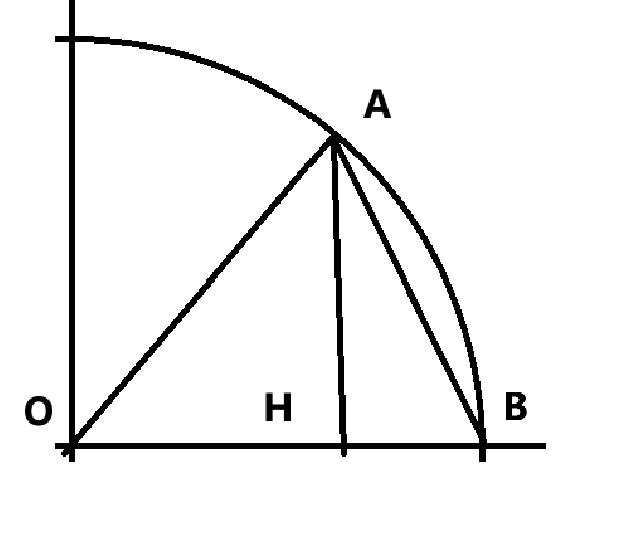
\includegraphics[width=7cm, height=6cm]{images/trig_function_lemm.png}
    
    Возьмем какую-то точку $H$ так, что $\angle AOB = x$. Посчитаем $S_{\Delta AOB}$. $OB = 1$. Поэтому $S_{\Delta AOB} = \cfrac{AH \cdot OB}{2} = \cfrac{\sin x}{2}$. Посчитаем площадь сегмента. Найду $S_{\text{сегмент}} = \pi r^2 * \frac{x}{2\pi}$ = $\cfrac{x}{2}$. Дострою за точку $A$ до прямоугольного треугольника. Получу $S_{\Delta} = \cfrac{\tg x}{2}$, откуда я и получаю нужное мне неравенство.
\end{enumerate}

 \sout{что же такое эта ваша площадь, узнаете во втором семестре БУ.}

\textbf{Следствие.} $\sin x, \cos x$ - непр. функции на $\mathbb{R}$

$|\sin x - \sin x_0| = |2 \sin \cfrac{x-x_0}{2}\cdot \cos {x+x_0}/2| \leq 2 \sin \cfrac{|x-x_0|}{2}\leq  \cfrac{2|x-x_0|}{2} $. То есть предел существует, откуда непрерывна. Ну а косинус~--- сдвинутый синус.

\textbf{Следствие.} $\lim\limits_{x\shortrightarrow 0} \cfrac{\sin x}{x} = 1$. Достаточно доказать, что предел с одной стороны.
\begin{enumerate}
    \item[] \prooff{}
    При $x \in (0,\cfrac{\pi}{2}): \cos x< \cfrac{\sin x }{x}<1$. По принципу двух городовых середина стремится к 1. (Равенство посередине~--- переписанное равенство сверху).
\end{enumerate}

\textbf{Следствие.} $\sin x$ дифференцируема при всех $x \in \mathbb{R}$, $(\sin x)' = \cos x$.

$\lim\limits_{h\shortrightarrow 0} \cfrac{\sin(x+h) -\sin x}{h} = \lim\limits_{h \shortrightarrow 0} \cfrac{2 \sin \cfrac{h}{2}\cdot \cos (x+ \cfrac{h}{2})}{h} = \lim \limits_{h\shortrightarrow 0} \cos (x+\cfrac{h}{2}) = \cos x$.

Откуда производная синуса такая. \sout{Кохась: синус найдите сами.}

\pagebreak
\subsection{Теоремы о среднем.}

\sout{предельно аккуратно со всем. Техал по звуку}

\thmm{Лемма.} $f: \langle a,b \rangle \shortrightarrow \mathbb{R}$, функция дифф в $x_0$, $f'(x_0)>0$.

Тогда $\exists \varepsilon>0 : f(x) >f(x_0)$, при $x\in (x_0,x_0 + \varepsilon)$, $f(x)< f(x_0),$ при $x \in (x_0-\varepsilon,x_0)$

\begin{enumerate}
    \item[] \prooff{}
    $\lim\limits_{x \shortrightarrow x_0} \cfrac{f(x)-f(x_0)}{x-x_0}= f(x_0)>0$. Смотрим на последовательность с правой стороны. По теореме о стабилизации знака, существует $\varepsilon$, такой, что  в окрестностях $\cfrac{f(x)-f(x_0)}{x-x_0}= f(x_0)>0$. Аналогично и с другой стороны есть такой $
    \varepsilon$, берем минимум и выигрываем (пристально посмотрите на числитель)
 
\end{enumerate}

\thmm{Теорема (Ферма)}

Пусть $f: \langle a,b\rangle \shortrightarrow \mathbb{R}$, $x_0 \in (a,b)$, $x_0$~--- точка максимума на интервале $(a,b)$, $x_0$ - дифференцируема в $x_0$. Тогда $f'(x_0) = 0$.

\begin{enumerate}
    \item[] \prooff{}
    Берем лемму. Если $f'(x_0) > 0$~--- сломалось, если $f'(x_0)<0$~--- сломалось по лемме, а откуда $f'(x_0) =0$

\end{enumerate}
\sout{вот как это может быть теорема ферма, когда слово производная придумали в 19 веке, а ферма умер и уже сгнил в гробу тогда.}

\thmm{Теорема (Ролля)} 

$f: [a,b] \shortrightarrow \mathbb{R}$, дифф на $(a,b)$, $f(a) = f(b)$, $f$ непрерывна на $[a,b]$. Тогда существует $c \in (a,b): f'(c)=0$.
\begin{enumerate}
    \item[] \prooff{}
    $f $ - непрерывна на $[a,b]$, откуда $[a,b]$ - компактен, по теореме Вейельштрасса, существует максимум и минимум функции. Если максимум и минимум на концах, тогда скучная ситуация (отрезок). Иначе максимум или минимум есть на $(a,b)$, откуда по теореме Ферма в этой точке будет $f'(x_0)=0$.
\end{enumerate}

$f:\langle a,b\rangle \shortrightarrow \mathbb{R}$ - многочлен, $x_0 \in \langle a,b\rangle. f(x_0) =0 $. Тогда $x_0$ называют \deff{корнем кратности k}, если $f(x) = (x-x_0)^k \cdot g(x)$, где $g(x_0) \neq 0$ и $g$ --- многочлен.

\textbf{Зам.} Если $x_0$ корень кратности $k$ многочлена $f(x)$, тогда $x_0$ корень кратности $k-1$ у $f'(x)$~--- очевидно.

\thmm{Теорема.}

$L_n(x) = ((x^2-1)^n)^{(n)}$ --- n раз продифф~--- \textbf{Многочлены Лежандра}.

Тогда $L_n$ имееет ровно $n$ вещественных корней на $(-1,1)$.
\begin{enumerate}
    \item[] \prooff{}
    (Решали на практиках). 
    
    Доказательство очевидно(просто много раз используйте теорему Ролля, а также прошлое замечание)
\end{enumerate}

\thmm{Теорема (Лагранжа)}.

$f: [a,b] \shortrightarrow \mathbb{R}$, дифф. на $(a,b)$ Непрерывна на $[a,b]$. 

Тогда $\exists \, c \in (a,b): \cfrac{f(b)-f(a)}{b-a} = f'(c)$

\thmm{Теорема (Коши)}.

$f: [a,b] \shortrightarrow \mathbb{R}$, дифф. на $(a,b)$. Непрерывна на $[a,b]$.

$g: [a,b] \shortrightarrow \mathbb{R}$, дифф. на $(a,b)$. Непрерывна на $[a,b]$. $g'\neq 0$ на $(a,b)$.

Тогда $\exists c \in (a,b): \cfrac{f(b)-f(a)}{g(b)-g(a)} = \cfrac{f'(c)}{g'(c)}$.
\begin{enumerate}
    \item[] \prooff{}
    $F(x) = f(x) - k g(x)$. Подберем k так, что  $F(a) = F(b)$.

    $f(a) - k \cdot g(a) = f(b) - k \cdot g(b)$

    $\cfrac{f(a)-f(b)}{g(a) - g(b)} = k$, при этом, тк $g'\neq 0$ на $(a,b)$, то $g(a) \neq g(b)$ (иначе по теореме Ролля мы проиграем). Значит такое k существует.

    Теперь из этого следует, что $\exists c, что F'(c) = 0$, то есть. 
    $f'(c) -  k \cdot g'(c) = 0$. А это то, что от нас требуют.  
\end{enumerate}

\textbf{Замечание от Славы.} Теорема Коши~--- обобщение теоремы Лагранжа ($g(x) = x$).

\textbf{Следствие:} $f:\langle a,b\rangle \shortrightarrow \mathbb{R}$ дифф. на $(a,b)$. $\exists M>0: \forall k \in (a,b): |f'(k)| \leq M$.

Тогда для любых $x_0, x_0 + h \in \langle a,b \rangle$: $|f(x_0)-f(x_0+h)|\leq M \cdot |h|$.

\textbf{Следствие:} $f$~--- непрерывна на $[x_0, x_0+h]$, дифференцируема на $(x_0, x_0+h)$. $\lim\limits_{x\shortrightarrow x_0  +0} f'(x) = A \in \mathbb{R}$.  Тогда $f'_{+}(x_0) = A$
\begin{enumerate}
    \item[] \prooff{}
    $\lim\limits_{x \shortrightarrow x_0 + 0} \cfrac{f(x)-f(x_0)}{x-x_0} = \lim\limits_{x\shortrightarrow x_0} f'(c)$, где $c = c(x) \in (x_0,x)$, определенно теоремой Лагранжа.
    Откуда очевидно.
\end{enumerate}

\thmm{Теорема (Дарбу, о промежуточном значении производной)}

$f: [a,b] \shortrightarrow \mathbb{R},$ дифф. $\shortrightarrow [a,b]$. Тогда $\forall C$ между $f'(a),f'(b)$, существует $c \in (a,b): f'(c) = C$.
\begin{enumerate}
    \item[] \prooff{}
$g(x) = f(x) - Cx$.

$g'(a) $ и $g'(b)$ \sout{что-то больше нуля, что-то меньше нуля. Значит есть точка принимающая ноль} - так нельзя, так как про непрерывность производной мы ничего не знаем.

Н.У.О $g'(a)>0, g'(b)<0$. Пусть $ c$ - точка максимума $g$ на $[a,b]$, она не может быть крайней по лемме в начале параграфа, откуда $g'(c) = 0$.
\end{enumerate}

\textbf{Следствие.} Если $f$ дифф на $\langle a,b \rangle $, тогда $f(\langle a,b \rangle)$~--- промежуток.

\textbf{Следствие.} $f' $ не имеет разрывов первого рода.
\pagebreak

\subsection{Школьный урок}

$x^\alpha, \alpha \in \mathbb{Q}$. Обозначается $f_{\alpha}(x) =x^\alpha$.

$\alpha = \mathbb{N}$.  Очевидно непрерывно на $\mathbb{R}$. Все понятно

$\alpha = -\mathbb{N}$. Обратная, непрерывность и существование везде кроме нуля и монотонно

$\alpha = 0$. Тождественная единица. $0^0 = 1$ ради непрерывности.

$\alpha = \cfrac{1}{n}$. n - нечет., тогда $f_n: \mathbb{R} \shortrightarrow \mathbb{R}$ --- непрерывная, строго монотонная, откуда есть обратная. Тогда  $f_{\frac{1}{n}}=f_n^{-1}$.

$\alpha = \cfrac{1}{n}$. n - чет., тогда $f_n: \mathbb{R} \shortrightarrow \mathbb{R}$ --- непрерывная, строго монотонная на $[0, +\infty)$ , откуда есть обратная на $[0, +\infty)$. Тогда  $f_{\frac{1}{n}}=f_n^{-1}$ на $[0, +\infty)$

$\alpha \in \mathbb{Q}, \alpha  = \cfrac{p}{q}, (p,q) =1$ $p \in \mathbb{Z}, q \in \mathbb{N}$, $f_\alpha = f_\frac{1}{q} \cdot f_p$.

\thmm{Теорема.} 

Число $e^2$~--- иррационально. [$e$ тоже будет рационально :)]

\begin{enumerate}
    \item[] \prooff{}
    Пусть $e^2 = \cfrac{2*k}{n}$. $n \cdot e = 2k \cdot e^{-1}$.

    $n(2k-1)! e = (2k)! e^{-1}$.

    $n(2k-1)! \cdot (1 + 1 + \frac{1}{2!} + \frac{1}{3!} + \ldots +\cfrac{1}{(2k-1)!}+ \cfrac{e^c}{(2k!)})$, $c \in (0,1)$~--- воспользовались разложением в форме Лагранжа в $0$ и подставили $1$.

    $=$ целое $+ \cfrac{n}{2k}\cdot e^c = $ целое + $\cfrac{e^c}{e^2}$.

    $(2k)! (1 - 1 + \cfrac{1}{2} + \cfrac{1}{2k!} - \cfrac{e^c}{(2k+1)!})$~--- воспользовались разложением в форме Лагранжа в $0$ и подставили $-1$.
    
    = целое $- \cfrac{e^c}{(2k+1)}$. И у нас не сходятся дробные части. В первом случае она меньше $\cfrac{1}{2}$, а во-втором случае больше $\cfrac{1}{2}$.
\end{enumerate}

 %Todo: 2.20 13 лекции кохась говорит что-то про метод ньютона я не осознал

 \deff{Метод Ньютона.}

Цель метода: Найти корень на промежутке $(a,b)$. (Мы берем приближение корня) 


 Беру точку $x_n$. Беру уравнение касательной в точке $x_n$ и еще точку $(x_{n+1})$, в которой эта прямая пересекает ось x. Пусть $\Psi$~--- точка  в которой находится корень, который мы ищем. Посмотрим, как близко мы к корню.

 $\Psi - x_{n+1} = \Psi-x_n + \cfrac{f(x_n)}{f'(x_n)} = \cfrac{f(x_n)  + f'(x_n) (\Psi-x_n)}{f'(x_n)}$.

 Посмотрим на разложение в Лагранже:
 
 $f(\Psi) = f(x_n) + \cfrac{f'(x_n)}{1!}(\Psi-x_n) + \cfrac{f''(c)}{2!}(\Psi-x_n)^2 = 0$.

$ \cfrac{f(x_n)  + f'(x_n) (\Psi-x_n)}{f'(x_n)} = -\cfrac{1}{2}\cdot \cfrac{f''(c)(1-x_n)}{f'(x_n)}$.

Возьмем $m = \min (f'(x))$, $M = \max |f''(x)| $. на нашем интервале

$|\Psi-x_{n+1}| = \cfrac{1}{2}\cdot \cfrac{|f''(c)(1-x_n)|}{|f'(x_n)|}(\Psi -x_n)^2\leq \frac{M}{2m}|\Psi - x_n|^2 \leq \frac{M}{2m}(\frac{M}{2m}|\Psi-{x_{n-1}}|^2)^2\leq \ldots \leq \frac{M}{2m}^{1+2+\ldots+2^{n+1}} |\Psi-x_1|^{2^n}= \frac{2m}{M}(\cfrac{M}{2m}|\Psi-x_1|)^{2^n}$.

Метод рабочий, если вам не выбрасывает никуда далеко.(Как я понял тут нет докзаательства)

\textbf{Замечание от Славы.} Буквально записал то, что говорил Кохась. Не могу придумать более адекватного объяснения

\pagebreak
\subsection{Производные ВЫСШЕГО порядка.}

$f:\langle a,b \rangle \shortrightarrow \mathbb{R}$ --- дифф на $\langle a,b \rangle$. $x_0 \in \langle a,b \rangle$,  Если функция $f'(x)$ дифф. в $x_0$. Тогда назовем $(f'(x_0))'$ --- \deff{второй производной} f в точке $x_0$.

Если $\forall x_0 \in \langle a,b\rangle$, то $f''(x)$~--- функция второй производной.

Аналогично $f^{(n)}(x_0)$, $n$-ая производная.

$\langle a,b\rangle$, $C^n (\langle a,b \rangle)$ --- множество функций, который n раз дифференцируемы на $(a,b)$ и $f^{(n)}$ непрерывна на $\langle a,b \rangle$

%TODO 2:11:00 12 лекции: происходит какой-то пиздец

\thmm{Теорема (Формула Тейлора с остатком в форме Пеано)}

$f: \langle a,b \rangle \shortrightarrow \mathbb{R}. x_0 \in \langle a,b \rangle$ $f - (n-1)$ раз дифф. на $\langle a,b \rangle$.

$\exists f^{(n)}(x_0) \in \mathbb{R}.$ Тогда:

$f(x) = \sum\limits_{k=0}^n  \cfrac{f^{(k)}(x_0)}{k!}(x-x_0)^k + o((x-x_0)^n) $, $x\shortrightarrow x_0$

\begin{enumerate}
    \item[] \prooff{}
    1) Начну с случая $f(x_0) = f'(x_0) =\ldots f^{(n)}(x_0)=0$.  Докажем, что $f(x) = 0 + o((x-x_0)^n) $, $x \shortrightarrow x_0$.

    \textbf{База:} $n=1$. $f(x) = f(x_0) + f'(x_0)(x-x_0) + o(x-x_0)$.
    
    \textbf{Переход:}  $n \shortrightarrow n+1$. Видно, что $f'$ удовл предположению индукции. Значит $f'(x) = o(x-x_0)^{n}$, $x \shortrightarrow x_0$. По теореме Лагранжа $f(x) - f(x_0) = f'(c)(x-x_0)$, где $c \in (x, x_0)$.

    $|\cfrac{f(x)}{(x-x_0)^{n+1}}| = |\cfrac{f(x) - f(x_0)}{(x-x_0)^{n+1}}| = |\cfrac{ f'(c)(x-x_0)}{(x-x_0)^n}|= |\cfrac{f'(c)}{(c-x_0)^n}| \cdot |\cfrac{(c-x_0)^n}{(x-x_0)^n}| \shortrightarrow 0$ --- победили.

    2) Общий случай. Рассмотрим $g(x) = f(x) - T_n(f,x_0) = f(x) - (\sum\limits_{k=0}^n  \cfrac{f^{(k)}(x_0)}{k!}(x-x_0)^k)$. Заметим, что $g(x_0) = 0$,\ldots, $g^{(n)}(x_0)=0$. Используем частный, откуда и получаем нужное.

    %TODO: !спросить про то, как дифференцироваь о малое.
\end{enumerate}

\thmm{Теорема (Формула Тейлора с остатком в форме Лагранжа)}

$f \in C^n(\langle a,b \rangle )$, f - $(n+1)$ раз дифференцируемы на $(a+b)$

%TODO: спросить у кохася

$x, x_0 \in \langle a,b\rangle$. Тогда $\exists c \in (x, x_0)$.

$f(x) = \sum\limits_{k=0}^n  \cfrac{f^{(k)}(x_0)}{k!}(x-x_0)^k + \cfrac{f^{(n+1)}(c)}{(n+1)!}(x-x_0)^{n+1} $
\begin{enumerate}
    \item[] \prooff{}

    $\phi(t) = f(x) - \sum\limits_{k=0}^n \cfrac{f^{k}(t)}{k!}(x-t)^k$. Позамечаем интересные вещи.

    $\phi(x) = 0$, $\phi(x_0) = $ остаток в формуле Тейлора.

    $\phi'(t) = - \cfrac{f^{n+1}(t)}{n!}(x-t)^n$

    \textbf{Теорема Коши.} $\cfrac{f(b)-f(a)}{g(b)-g(a) } = \cfrac{f'(x)}{g'(x)}$. $f = \phi$, $g(t) = (x-t)^{n+1}$, $a= x_0$, $b=x$;

    $\cfrac{\phi(x)-\phi(x_0)}{g(x)-g(x_0)} = \cfrac{-R_{n+1}(x_0)}{-(x-x_0)^{n+1}} = \cfrac{-\cfrac{f^{(n+1)}(c)}{n!} (x-c)^n}{-(n+1) (x-c)^n}$

    Откуда и получаем наш вид остатка
    %TODO: !спросить про то, как дифференцироваь о малое.
\end{enumerate}

\textbf{Замечание от Славы.} Кохась вдруг стал обозначать остаток многочлена Тейлора как $R_{n+1}(x_0)$.

\textbf{Замечание.} Пусть $f\in C^{\infty}(\langle a,b\rangle)$. Пусть существует $ M,A$:

$\forall t \in \langle a,b \rangle: |f^{n}(t)|\leq MA^n$.

Тогда $\forall x.x_0 \in \langle a,b\rangle$. $T_n(f,x_0)(x) \shortrightarrow f(x)$, при $n \shortrightarrow +\infty$. Доказательство это просто аккуратные оценки.

\textbf{Замечание.} $f(x) = x + x^2 + x^3 \cdot \sin(\cfrac{1}{x^{100}})$, при $x\shortrightarrow 0$ ~--- продифференцируйте и поймите, что с вашей жизнью не так.

Асимптотическое разложение просто опасно дифференцировать.

$f(x) = a_0+a_1x +\ldots +a_n x^n + o(x^n)$~--- формула Тейлора, $x_0=0$.

То $f'(x) = a_1+2a_2x + \ldots + n a_n x^{n-1} + o(x^{(n-1)})$ ~--- верная формула, так еще и формула тейлора для $f'$.

\thmm{Теорема.}

Пусть $P(x), Q(x) $ - многочлен, $\deg P(x) < \deg Q(x)$, $P(x),Q(x)$ --- взаимнопросты.

$Q(x) = (x-x_1)^{\alpha_1}\cdot (x-x_2)^{\alpha_2}\ldots(x-x_n)^{\alpha_n}$.

Тогда существуют вещественные числа $A_1, A_2,\ldots, A_{\alpha_1}$, $B_1,\ldots, B_{\alpha_2},\ldots, D_{1},\ldots, D_{\alpha_n}$, что

\[\cfrac{P(x)}{Q(x)}=\Big(\cfrac{A_1}{x-x_1}+ \ldots + \cfrac{A_{\alpha_1}}{(x-x_1)^{\alpha_1}}\Big) +\Big(\cfrac{B_1}{x-x_2}+ \ldots + \cfrac{B_{\alpha_2}}{(x-x_2)^{\alpha_2}}\Big) +\]

\[ \ldots + \Big(\cfrac{D_1}{x-x_n}+ \ldots + \cfrac{D_{\alpha_n}}{(x-x_n)^{\alpha_n}}\Big)\]

\begin{enumerate}
    \item[] \prooff{}
    Пусть $F_1(x) = \cfrac{P(x)}{Q(x)}(x-x_1)^{\alpha_1} = \cfrac{P(x)}{(x-x_2)^{\alpha_2}\ldots(x-x_n)^{\alpha_n}}$.

    Разложим $F_1$ по формуле Тейлора в точке $x_1$:

    $F_1(x) = a_0 + a_1(x-x_1) + \ldots + a_{\alpha_1}(x-x_1)^{\alpha_1}+o((x-x_1)^{\alpha_1})$.

    $\cfrac{P(x)}{Q(x)} = \cfrac{F_1(x)}{(x-x_1)^{\alpha_1}} = \cfrac{a_0}{(x-x_1)^{\alpha_1}} + \cfrac{a_1}{(x-x_1)^{\alpha_1-1}}+\ldots + \cfrac{a_{\alpha_1-1}}{(x-x_1)} + a_{\alpha_1}+o(1)$, $x\shortrightarrow x_1$.

    $A_1 = \alpha_1-1$  и так далее.

    Аналогично с другими $B,\ldots, D$. Построили. Почему получили то, что надо

    $\cfrac{P(x)}{Q(x)}-\Big(\cfrac{A_1}{x-x_1}+\ldots + \cfrac{A_{\alpha_1}}{(x-x_1)^{\alpha_1}}\Big)-\ldots -\Big(\cfrac{D_1}{x-x_n}+ \ldots + \cfrac{D_{\alpha_n}}{(x-x_n)^{\alpha_n}}\Big)$.

    Давайте посмотрим на первую пару. Получается что-то ограниченное при $x\shortrightarrow x_1$. Но как такое может быть, это значит то, что было в знаменателе: $(x-x_1)^{\alpha_1}$--- сократилось! Значит у меня сокращается весь знаменатель, если я вычту все серии.

    Значит такая разность на самом деле функция у которой сократился весь знаменатель. Это многочлен. Но как такое может быть $\deg P<\deg Q$. Откуда это просто 0.(тут надо больше аккуратности).
\end{enumerate}



















\pagebreak
\subsection{Показательные функции}

Хочу найти все непрерывные функции такие, что$f(x+y) = f(x) \cdot f(y) $. Назову все такие функции \deff{показательными} (игнорирую тождественный ноль и тождественный один).

\textbf{Свойства.}

\begin{enumerate}
    \item $\forall x: f(x) > 0; f(0) = 1$. Очевидно откуда
    \item $\forall r \in \mathbb{Q}: \forall x: f(rx) = f(x)^r$. Очевидно из определения рациональных степеней.
    \item Введем число $a=f(1)$,  f - строго монотонная, более того: $a\neq 1$. Если $a>1$,  то строго возрастает. Если $a<1$, то строго убывает. Доказательство очевидно.
    \item Множество значений это $(0,+\infty)$. Очевидно по свойствам степени.  
    \item Зафиксируем функцию. Пусть существует функция $\overline{f}$, которая в f(1) принимает то же самое значение. Заметим, что $\overline{f}=f$.
\end{enumerate}
    


\sout{Кохась: возьму кредит в виде теоремы.}

\thmm{Теорема.}

$\exists f_0$ - показательная  функция, такая что:

$\lim\limits_{x \shortrightarrow 0} \cfrac{f_0(x)-1}{x}=1$

\sout{Кохась: ну пока пофиг что такая может не  существовать. Пока что-нибудь подоказываем }

\thmm{Теорема.}

$\exists \alpha \in \mathbb{R}: \forall x \in \mathbb{R}: f(x)=f_0(\alpha x)$


\begin{enumerate}
    \item[] \prooff{}
     $f(1) = a > 0$; $f_0(\alpha) = a$, $\alpha \neq 0$.

     Посмотрим на $g(x) = f_0(\alpha x)$ -  это показательная функция (удовлетворяет определению). $g(1) = a = f(1)$, откуда по свойству 5 они совпадают. 
\end{enumerate}

Что мы только доказали: Любую показательную функцию можно выразить через $f_0$.

\textbf{Следствие:} функция из теоремы 2 - единственна (если существует). (От прот.)

Функцию $f_0(x)$ буду называть \deff{экспонентой}. Буду обозначать ее $f_0(x) = exp(x) = e^x$. (пока это не то е, это просто обозначение). 

Так как $\cfrac{e^x - 1}{x}\shortrightarrow 1$, откуда $e^x >1$, при $x>0$.

\textbf{Следствие}. $a>0, a\neq 1$ $\exists! $ показ. функция $f(1) = a$. Очевидно

Обозначим все наши функции: $a^x$

\textbf{Следствие}. $\forall x,y: \forall a>0, a \neq 1: a^{xy} = (a^x)^y  = (a^y)^x$. 

$a>0,a \neq 1, a^x: \mathbb{R} \shortrightarrow (0, +\infty)$ строго монот., непрерывно. Откуда существует обратная. Назовем ее \deff{логарифмом}. $\ln x = \log_e x$.

\textbf{Замечательный предел.} $\lim\limits_{x \shortrightarrow 0} \cfrac{e^x-1}{x}=1$

\textbf{Следствие.} $(e^x)' = \lim\limits_{h\shortrightarrow 0} \cfrac{e^{x+h}-e^x}{h}=e^x$

\textbf{Замечательный предел.} $\lim\limits_{x\shortrightarrow 0} \cfrac{\ln(1+x)}{x}=1 $. Переверните дробь и увидите что-то больно похожее на первый зам. предел.

\textbf{Следствие.} $(\ln x)' = \lim \limits_{h \shortrightarrow 0} \cfrac{\ln(x+h)-\ln x}{h} = \lim \cfrac{\ln(1+ \frac{h}{x})}{\frac{h}{x}}\cdot \cfrac{1}{x} = \cfrac{1}{x}$

\textbf{Замечательный предел.} $\lim\limits_{x\shortrightarrow 0} (1+x)^{\frac{1}{x}}=e$. $e^{\ln (1+x) \frac{1}{x}}\shortrightarrow e$.

\textbf{Следствие.}  Старое e и новое e совпадают, потому что старое e это предел $(1+\frac{1}{n})^n$.

\textbf{Замечательный предел.} $\lim\limits_{x\shortrightarrow 0} \cfrac{(1+x)^\alpha-1}{x} = \alpha$.

$\cfrac{(1+x)^\alpha}{x}=\cfrac{f(x)}{x}=\cfrac{f(x)}{\ln(f(x)+1)} \cdot \cfrac{\alpha \ln(1+x)}{x}\shortrightarrow \alpha$.
\pagebreak


\subsection{Монотонность и экстремумы.}

\thmm{Теорема (Критерий монотонности)}

$f \subset С(\langle a,b\rangle)$, дифф на $(a,b)$. Тогда f возрастает на $\langle a,b\rangle \Leftrightarrow f' \geq 0$ на $(a,b)$

Доказательство очевидно. (Аналогично убывание)

\textbf{Следствие.} $f: \langle a,b\rangle \shortrightarrow \mathbb{R}$.  Тогда $f = const \Leftrightarrow f \in C(\langle a,b \rangle)$ и $f$ - дифф на интервале, $f'=0$. Очевидно.

\textbf{Следствие.} $f\in C(\langle a,b \rangle),$ дифф на $(a,b)$. Тогда $f$ - строго возрастающая $\Leftrightarrow$

\begin{enumerate}
    \item $f'\geq 0$ на $(a,b)$.
    \item ни на каком промежутке $\langle x_1,x_2\rangle \subset \langle a,b \rangle, f' \neq 0 $ на $\langle x_1,x_2 \rangle$. (интервал не из одной точки).
\end{enumerate}

Доказательства очевидное

\textbf{Следствие.} $f,g \in C(\langle a,b\rangle)$, дифф на $\langle a,b)$. Пусть $f(a)< g(a)$, а еще $f'(x)<g'(x)$ на $(a,b)$. Тогда $f(x)\leq g(x) $ на $\langle a,b\rangle$. Доказательство очевидно (Посмотреть на $h(x) = g(x)-f(x)$)

$f: X \shortrightarrow \mathbb{R}$, $x_0$ --- \deff{точка лок. максимума}. Cуществует Окрестность точки $x_0: \forall x \in U(x_0): f(x)\leq f(x_0)$. \deff{Экстремум.}

\thmm{Теорема (о необходимом и достаточном условии экстремума)}

$f: \langle a,b \rangle \shortrightarrow \mathbb{R}$. $x_0 \in (a,b)$. Пусть $f$ - дифф. $(a,b)$. Тогда:

\begin{enumerate}
    \item $x_0$ --- экстремум $\Rightarrow f'(x_0) = 0$.
    \item $f$ --- n раз дифф в $x_0$. Пусть $f'(x_0)=f''(x_0)=\ldots =f^{(n-1)}(x_n)=0$, $f^{(n)}\neq 0$. Если $f^{(n)}(x_0)>0,$ n - четная, тогда минимум. Если нечетная, то не экстремум. Если   $f^{(n)}(x_0)<0$, n - четная, тогда максимум. Если нечетная, то не экстремум.
\end{enumerate}

\begin{enumerate}
    \item[] \prooff{}
    1) Теорема Ферма.

    2) $f(x) = \sum\limits_{k=0}^n \cfrac{f^{(k)}(x_0)}{k!}(x-x_0)^k + o((x-x_0)^n)$, при $x\shortrightarrow x_0$ --- разложение Тейлора.

    $f(x) -f(x_0)= \cfrac{f^{(n)}(x_0)}{n!}(x-x_0)^n + o((x-x_0)^n)$ по условию.

    $=\cfrac{f^{n}(x_0)}{n!}(x-x_0)^n + (x-x_0)^n \alpha(x)$, где $\alpha(x) \shortrightarrow 0 $  при $x\shortrightarrow x_0$ - остаток в форме Пеано.

    $= (\cfrac{f^{(n)}(x_0)}{n!} + \alpha(x))(x-x_0)^n$. Откуда уже методом вглядывания получится нужное нам выражение.
\end{enumerate}

\pagebreak
\subsection{Равномерная непрерывность.}

$f: X \shortrightarrow \mathbb{R}$. X - метрическое пространство. 

$f$ - \deff{равномерно непрерывно}, если

$\forall \varepsilon > 0: \exists \delta >0" \forall x_1,x_2 \in X: \rho(x_1,x_2)<\delta: |f(x_1)-f(x_2)|<|\varepsilon|$.

$f: \mathbb{R}\shortrightarrow \mathbb{R}, E\subset \mathbb{R}$, $f$ - равномерно непрерывно E.

$\forall \varepsilon >0: \exists \delta>0: \forall x_1,x_2 \in E: |x_1-x_2|<\delta: |f(x_1)-f(x_2)|< \delta$.

\textbf{Замечание.} $X \shortrightarrow Y$ м.п.-ства $\rho(f(x_1),f(x_2))<\varepsilon$. (Можно обобщить).

\thmm{Теорема (Кантора)}

Дано отображение $X \shortrightarrow Y$, $X$ - компактно, $f -$ непр на X.

Тогда $f -$ равномерно непр.

\begin{enumerate}
    \item[] \prooff{}
    От противного
   $\exists \varepsilon > 0: \forall \delta, \delta = \cfrac{1}{n}\,\, \exists \,x_n, \overline{x_n}<\cfrac{1}{n}: \rho(f(x_n),f(\overline{x_n}))>\varepsilon.$

   В метрическом пространстве $\Leftrightarrow$ секв. компактно. (почему?)

   Возьмем $x_n$ - последовательность. Есть сходящаяся подпоследовательность. Выберем. Тогда для $x_n$ начнет ломаться непрерывность ($x_n $ и $\overline{x_n}$ стремятся к a)
\end{enumerate}

\textbf{Следствие.} $f:[a,b] \shortrightarrow \mathbb{R}$, непр. Тогда f равномерно непрерывно.

\end{document}  